% !Mode:: "TeX:UTF-8"
\chapter{Mapping}
\label{cpt:12}
\begin{mdframed}  
	\textbf{Goal of Study}
	\begin{enumerate}[labelindent=0em,leftmargin=1.5em]
		\item Learn how to estimate the dense depth in monocular SLAM. 
		\item Implement the dense depth estimation in monocular SLAM.
		\item Learn some of the commonly used map forms in RGB-D reconstruction. 
	\end{enumerate}
\end{mdframed}

In this lecture, we start to introduce the algorithm of the mapping part. In the front and back ends, we focus on the problem of simultaneously estimating the camera motion trajectory and the spatial position of the feature points. However, in real applications, in addition to localizing the camera, there are many other requirements. For example, consider the SLAM on the robot, we would hope that the map can be used for positioning, navigation, obstacle avoidance and interaction. The feature point map obviously cannot meet all these needs. Therefore, in this lecture, we will discuss various forms of maps in more detail, and point out the shortcomings in current visual SLAM maps.

\newpage
\section{Brief Introduction}
Mapping should be one of the two goals of SLAM-because SLAM is called simultaneous positioning and mapping. But until now, we have been discussing the localization problems for long time, including localization through feature points, direct method, and back-end optimization. So, does this imply that mapping is not that important in SLAM, so we didn't discuss it until this lecture?

The answer is negative. In fact, in the classic SLAM model, what we call a map is a collection of all road signs. Once the location of the signpost is determined, it can be said that we have completed the mapping. Therefore, whether the aforementioned visual odometer or Bundle Adjustment is good, in fact, they both model the position of the road signs and optimize them. From this perspective, we have discussed the issue of mapping. So why do we need to list the map separately?

This is because people have different needs for mapping. As a kind of underlying technology, SLAM is often used to provide information for upper-layer applications. If the upper layer is a robot, then the developer of the application layer may want to use SLAM to do global positioning and let the robot navigate in the map-for example, a sweeper needs to complete the sweeping work, hoping to calculate a path that can cover the entire map. Or, if the upper layer is an augmented reality device, the developer may wish to superimpose the virtual object on the real object. In particular, it may also need to handle the occlusion relationship between the virtual object and the real object.

We found that the requirements for “positioning” at the application level are similar, and they hope that SLAM provides the camera or the spatial pose information of the subject carrying the camera. For maps, there are many different requirements. From the point of view of visual SLAM, "map" serves "positioning"; but from the perspective of application, "map" obviously has many other requirements. Regarding the usefulness of the map, we can roughly summarize it as follows:

\begin{enumerate}
	\item \textbf{Localization}. Localization is a basic function of the map. In the previous part of visual odometry, we discussed how to use local maps to achieve positioning. In the loop detection part, we also saw that as long as there is global descriptor information, we can also determine the position of the robot through loop detection. Furthermore, we also hope to save the map so that the robot can still locate on the map after the next startup, so that we only need to model the map once instead of doing a complete SLAM every time the robot is started.
	\item \textbf{Navigation}. Navigation refers to the process in which a robot can plan a path on a map, find a path between any two map points, and then control its movement to a target point. In this process, we need to know at least \textbf{Which places in the map are not passable and which places are passable}. This is beyond the capability of sparse feature point maps, and we must have another map form. We will say later that this must be at least a \textbf{dense} map.
	\item \textbf{Obstacle avoidance}. Obstacle avoidance is also a problem often encountered by robots. It is similar to navigation, but pays more attention to the handling of local and dynamic obstacles. Similarly, with only feature points, we cannot judge whether a feature point is an obstacle, so \textbf{dense} map is needed.
	\item \textbf{Reconstruction}. Sometimes, we hope to use SLAM to obtain the reconstruction of the surrounding environment. This kind of map is mainly used for demonstration, so we hope it looks more comfortable and beautiful. Or, we can also use the map for communication so that others can remotely watch the 3D objects or scenes we reconstructed-such as 3D video calls or online shopping. This kind of map is also \textbf{dense}, and we also have some requirements for its appearance. We may not be satisfied with the dense point cloud reconstruction, but hope to build a textured plane, just like the three-dimensional scene in a video game.
	\item \textbf{Interaction}. Interaction mainly refers to the interaction between people and the map. For example, in augmented reality, we will place virtual objects in the room and interact with these virtual objects-for example, I will click on the virtual web browser on the wall to watch the video, or Throw objects on the wall, hoping that they will have a (virtual) physical collision. On the other hand, there will also be interactions with people and maps in robot applications. For example, the robot may receive the command "take the newspaper on the table". Then, in addition to the environment map, the robot also needs to know which map is the "table", what is called "above", and what is called "newspaper". This requires robots to have a higher level of knowledge of maps-also known as semantic maps.
\end{enumerate}

\autoref{fig:maps} visually explains the relationship between the various map types discussed above and their uses. Our previous discussion basically focused on the "sparse feature map" part, and did not discuss dense maps. The so-called dense map is relative to the sparse map. The sparse map only models the part of interest, that is, the feature points (signpost points) that have been mentioned for a long time. The dense map refers to the part that has been seen by modeling \textbf{all}. For the same table, the sparse map may only model the four corners of the table, while the dense map will model the entire desktop. Although from the perspective of positioning, a map with only four corners can also be used to locate the camera, but since we cannot infer the spatial structure between these points from the four corners, it is impossible to complete navigation with only four corners. , Obstacle avoidance and other tasks that require dense maps to complete.

\begin{figure}[!ht]
	\centering
	\includegraphics[width=1.0\textwidth]{mapping/maps.pdf}
	\caption{Different maps from \cite{Mur-Artal2015, Labbe2014, Salas-Moreno2013}.}
	\label{fig:maps}
\end{figure}

As can be seen from the above discussion, the dense map occupies a very important position. So, the remaining question is: Can a dense map be established through visual SLAM? If so, how to build it?

\section{Monocular Dense Reconstruction}
\subsection{Stereo Vision}
The dense reconstruction of visual SLAM is the first important topic of this lecture. Cameras have long been considered as bearing-only sensors. The pixels in a single image can only provide the angle between the object and the camera's imaging plane and the brightness collected by the object, but not the distance (range) of the object. In dense reconstruction, we need to know the distance of each pixel (or most of the pixels). There are roughly the following solutions for this:
\begin{enumerate}
	\item Use monocular cameras and estimate the depth using triangulation after motion. 
	\item Use stereo cameras by its disparity (similar for more than two eyes). 
	\item Use the depth sensor in RGB-D cameras to directly get the depth. 
\end{enumerate}

The first two methods are sometimes called stereo vision, and the moving monocular is also called moving view stereo (MVS). Compared with the depth measured directly by RGB-D, the acquisition of depth by monocular and binocular is often \textit{fragile}-we need to spend a lot of calculations, and finally get some unreliable depth estimation. Of course, RGB-D also has some limits on range, application range and illumination, but compared to monocular and binocular results, using RGB-D for dense reconstruction is often a more common choice. The advantage of monocular and binocular is that in outdoor and large scenes where RGB-D is not yet well applied, depth information can still be estimated through stereo vision.

Having said that, in this section we will lead readers to realize a single-purpose dense estimation and experience why it is thankless. Let’s start with the simplest case: how to estimate the depth of an image based on a video sequence over a period of time based on a given camera trajectory. In other words, we do not consider SLAM, first consider the slightly simpler mapping problem.

Assuming that there is a video sequence, we get the trajectory corresponding to each frame through some magic (of course, it is also probably estimated by the front-end of the visual odometer). Now we use the first image as the reference frame to calculate the depth (or distance) of each pixel in the reference frame. First of all, please remember how we completed the process in the feature matching section:

\begin{enumerate}
	\item First, we extract features from the image and calculate the matching between the features based on the descriptor. In other words, through the feature, we track a certain spatial point and know its position between each image.
	\item Then, since we cannot determine the position of the feature point with only one image, we must estimate its depth through observations under different viewing angles. The principle is the triangulation mentioned above.
\end{enumerate}

\subsection{Epipolar Line Search and Block Matching}
Let's first discuss the geometric relationship produced by observing the same point from different perspectives. This is very similar to the epipolar geometry discussed in section ~\ref{sec:epipolar-geometry}~. Please see \autoref{fig:epipolar-line-search}~. The camera on the left has observed a certain pixel $\bm{p}_1$. Since this is a monocular camera, we have no way of knowing its depth, so assuming that the depth may be within a certain area, it may be said that it is between a certain minimum and infinity: $(d_\mathrm{min}, +\ infty)$. Therefore, the spatial points corresponding to the pixel are distributed on a certain line segment (a ray in this example). From another perspective (the camera on the right), the projection of this line segment also forms a line on the image plane, which we know is called \textbf{polar line}. When the movement between the two cameras is known, this epipolar line can be determined\footnote{On the contrary, if the movement is not known, the epipolar line cannot be determined. }. Then the question is: Which point on the epipolar line is the $\bm{p}_1$ point we just saw?

\begin{figure}[!htp]
	\centering
	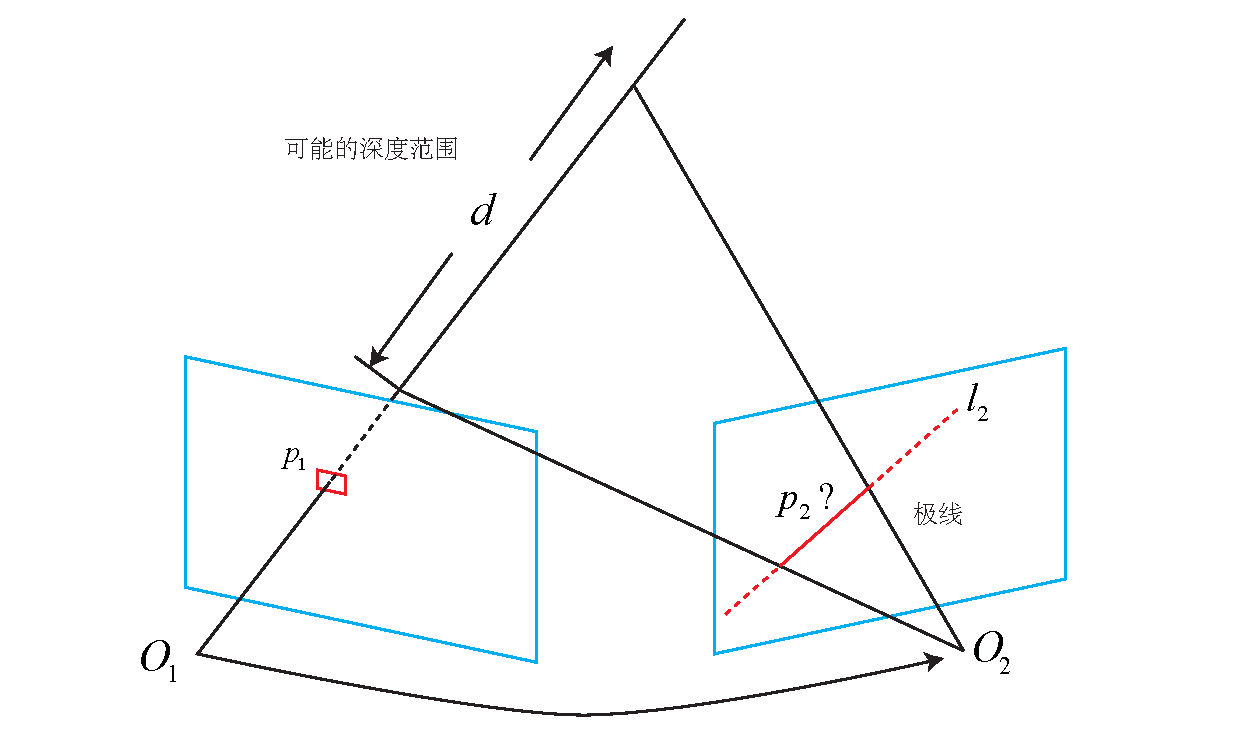
\includegraphics[width=.8\textwidth]{mapping/epipolar-line-search.pdf}
	\caption{Epipolar line search.}
	\label{fig:epipolar-line-search}
\end{figure}

Again, in the feature matching method, we find the position of $\bm{p}_2$ through features. However, now we don’t have a descriptor, so we can only search for points that are similar to $\bm{p}_1$ on the epipolar line. To be more specific, we may walk along one end of the epipolar line in the second image to the other, and compare the similarity of each pixel to $\bm{p}_1$ one by one. From the point of view of directly comparing pixels, this approach is the same as the direct method.

In the discussion of the direct method, we know that comparing the brightness value of a single pixel is not necessarily stable and reliable. One obvious thing is: if there are many similarities to $\bm{p}_1$ on the pole, how can we determine which one is true? This seems to return to the question we mentioned in the loop detection: how to determine the similarity of two images (or two points)? Loop detection is solved by bag of words, but because there are no features here, we have to find another way.

An intuitive idea is: Since the brightness of a single pixel is not distinguishable, can it be possible to compare pixel blocks? We take a small block of size $w \times w$ around $\bm{p}_1$, and then take many small blocks of the same size on the epipolar line for comparison, which can improve the discrimination to a certain extent . This is the so-called \textbf{block match}. Note that in this process, this comparison is meaningful only if the gray value of the entire small block remains unchanged between different images. Therefore, the assumption of the algorithm has changed from the gray invariance of pixels to the gray invariance of image blocks-to a certain extent, it has become stronger.

Okay, now we have taken the small blocks around $\bm{p}_1$, and also many small blocks on the epipolar line. May wish to record the small blocks around $\bm{p}_1$ as $\bm{A} \in \mathbb{R}^{w \times w}$, and record the $n$ small blocks on the extreme line Into $\bm{B}_i, i=1, \cdots, n$. So, how to calculate the difference between a small block and a small block? There are several different calculation methods:

\begin{enumerate}
	\item SAD (Sum of Absolute Difference):
	\begin{equation}
		S( \bm{A}, \bm{B} )_{\mathrm{SAD}} = \sum_{i,j} | \bm{A}(i,j) - \bm{B}(i,j) |.
	\end{equation}
	\item SSD (Sum of Squared Distance), not solid state drive:
	\begin{equation}
		S( \bm{A}, \bm{B} )_{\mathrm{SSD}} = \sum_{i,j} \left( \bm{A}(i,j) - \bm{B}(i,j) \right)^2.
	\end{equation}
	\item NCC (Normalized Cross Correlation):
	\begin{equation}
		S( \bm{A}, \bm{B} )_{\mathrm{NCC}} = \frac{{\sum\limits_{i,j} {\bm{A}(i,j)\bm{B}(i,j)} }}{{\sqrt {\sum\limits_{i,j} {\bm{A}{{(i,j)}^2}\sum\limits_{i,j} {\bm{B}{{(i,j)}^2}} } } }}.
	\end{equation}
	Please note that since correlation is used here, correlation close to 0 means that the two images are not similar, and close to 1 means similar. The first two distances are reversed. Close to 0 means similarity, while a larger value means dissimilar.
\end{enumerate}

Like many situations we have encountered, these calculation methods often have a contradiction between accuracy and efficiency. Methods with good accuracy often require complex calculations, while simple and fast algorithms often do not work well. This requires us to make a choice in actual engineering. In addition, in addition to these simple versions, we can \textbf{remove the mean of each small block first}, which is called averaging SSD, averaging NCC, and so on. After removing the mean value, we allow situations like "a small piece of $\bm{B}$ is brighter than $\bm{A}$ as a whole, but still very similar" \footnote{The overall lighter may be brighter by the ambient light Or the camera exposure parameters increase. }, so it is more reliable than before. If readers are interested in more block matching measurement methods, it is recommended to read the literature \cite{stereo-matching-website, Hirschmuller2007} as supplementary material.

Now, we have calculated the similarity measure between $\bm{A}$ and each $\bm{B}_i$ on the epipolar line. For the convenience of description, suppose we use NCC, then we will get an NCC distribution along the epipolar line. The shape of this distribution depends heavily on the image data, as shown in \autoref{fig:matching-score}~. In the case of a long search distance, we usually get a non-convex function: this distribution has many peaks, but there must be only one true corresponding point. In this case, we tend to use probability distributions to describe depth values, rather than using a single value to describe depth. Therefore, our question turns to how the depth distribution we estimate will change when we continue to search for different images with epipolar lines-this is the so-called \textbf{depth filter}.

\begin{figure}[!htp]
	\centering
	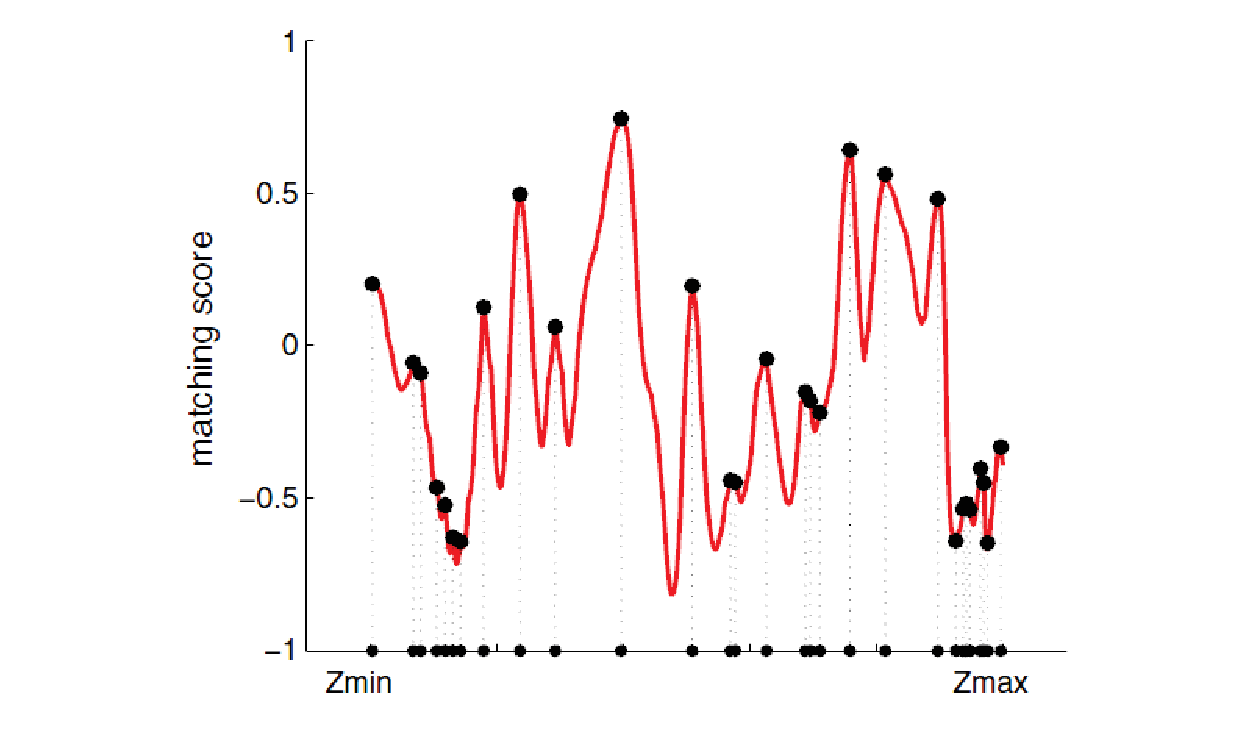
\includegraphics[width=.75\textwidth]{mapping/matching-score.pdf}
	\caption{Matching score along with the epipolar line. Figures are from \cite{Vogiatzis2011}.}
	\label{fig:matching-score}
\end{figure}

\subsection{Gaussian Depth Filters}
The estimation of pixel depth itself can also be modeled as a state estimation problem, so there are naturally two ways of solving the problem of filter and nonlinear optimization. Although the effect of non-linear optimization is better, in the case of strong real-time requirements such as SLAM, considering that the front-end has already occupied a lot of calculations, the filter method with less calculation is usually used in mapping. This is also the purpose of the depth filter discussion in this section.

There are several different ways of assuming the distribution of depth. First of all, under relatively simple assumptions, we can assume that the depth value obeys the Gaussian distribution, and get a Kalman-like method (but in fact it is just a normalized product, as we will see later). On the other hand, in \cite{Vogiatzis2011, Forster2014} and other documents, the assumption of uniform-Gaussian mixture distribution is also used to derive another form of more complex depth filter. Based on the principle of simplicity and ease of use, we first introduce and demonstrate the depth filter under the assumption of Gaussian distribution, and then take the filter with uniform-Gaussian mixture distribution as an exercise.

Assume the depth $d$ of a certain pixel satisfy:
\begin{equation}
	P(d) = N(\mu, \sigma^2).
\end{equation}

And whenever new data arrives, we will observe its depth. Similarly, suppose this observation is also a Gaussian distribution:
\begin{equation}
	P(d_{\mathrm{obs}}) = N(\mu_{\mathrm{obs}}, \sigma_{\mathrm{obs}}^2 ).
\end{equation}

Therefore, our question is how to use the observed information to update the original distribution of $d$. This is exactly an information fusion problem. According to Appendix A, we understand that the product of two Gaussian distributions is still a Gaussian distribution. Suppose the distribution of $d$ after fusion is $N(\mu_{\mathrm{fuse}}, \sigma_{\mathrm{fuse}}^2)$, then according to the product of the Gaussian distribution, there are:
\begin{equation}
	{\mu _{\mathrm{fuse}}} = \frac{{\sigma _{\mathrm{obs}}^2\mu  + {\sigma ^2}{\mu _{\mathrm{obs}}}}}{{{\sigma ^2} + \sigma _{\mathrm{obs}}^2}},\quad \sigma _{\mathrm{fuse}}^2 = \frac{{{\sigma ^2}\sigma _{\mathrm{obs}}^2}}{{{\sigma ^2} + \sigma _{\mathrm{obs}}^2}}.
\end{equation}

Since we only have observation equations and no motion equations, the depth here only uses the information fusion part, and there is no need to predict and update like the complete Kalman (of course, you can think of it as "the equation of motion is fixed for the depth value "Kalman filter). It can be seen that the fusion equation is indeed relatively simple and easy to understand, but the question remains: how to determine the distribution of the depth we observe? That is, how to calculate $\mu_{\mathrm{obs}}, \sigma_{\mathrm{obs}}$?

Regarding $\mu_{\mathrm{obs}}, \sigma_{\mathrm{obs}}$, there are also some different processing methods. For example, the document \cite{Engel2013} considers the sum of geometric uncertainty and photometric uncertainty, while \cite{Vogiatzis2011} only considers geometric uncertainty. For the time being, we only consider the uncertainty caused by geometric relations. Now, suppose we have determined the projection position of a pixel in the reference frame in the current frame through epipolar search and block matching. So, how much uncertainty does this position have on the depth?

Take \autoref{fig:uncertainty-mapping}~ as an example. Considering a certain epipolar search, we found the $\bm{p}_2$ point corresponding to $\bm{p}_1$, and thus observed the depth value of $\bm{p}_1$. We consider the three-dimensional point corresponding to $\bm{ p}_1$ is $\bm{P}$. We denote that $\bm{O}_1 \bm{P}$ is $\bm{p}$, and $\bm{O}_1 \bm{O}_2$ is the camera's translation $\bm{t} $, $\bm{O}_2 \bm{P}$ is denoted as $\bm{a}$. And, let the bottom two corners of this triangle be $\alpha, \beta$. Now, consider that there is a pixel size error on the epipolar line $l_2$, so that the angle of $\beta$ becomes $\beta'$, and $\bm{p}_2$ also becomes $\bm{p }_2'$, and remember the upper corner as $\gamma$. What we want to ask is, how big a difference between $\bm{p}'$ and $\bm{p}$ will be caused by this one pixel error?

\begin{figure}[!ht]
	\centering
	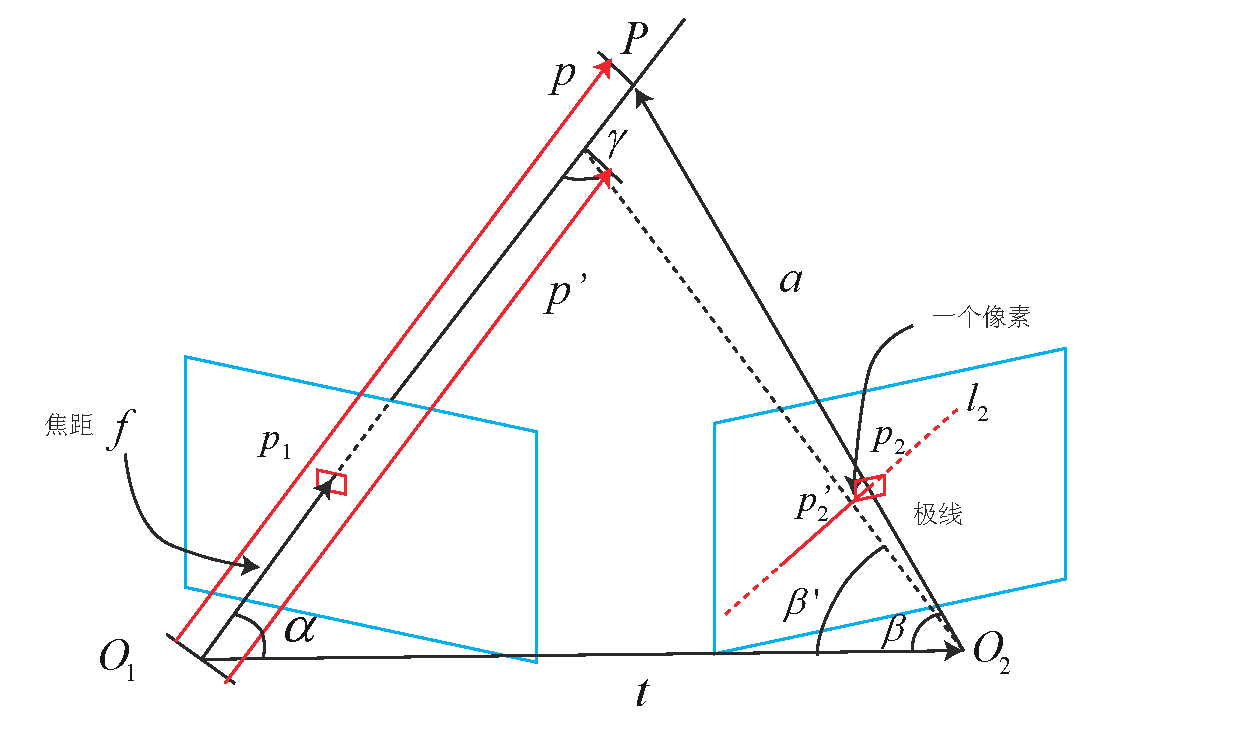
\includegraphics[width=.84\textwidth]{mapping/uncertainty.pdf}
	\caption{Uncertainty analysis.}
	\label{fig:uncertainty-mapping}
\end{figure}

This is a typical geometric problem. Let's list the geometric relationship between these quantities. Obviously:
\begin{equation}
	\begin{array}{l}
		\bm{a} = \bm{p} - \bm{t} \\
		\alpha  = \arccos \left\langle {\bm{p}, \bm{t}} \right\rangle \\
		\beta  = \arccos \left\langle {\bm{a}, - \bm{t}} \right\rangle .
	\end{array}
\end{equation}

Perturbing $\bm{p}_2$ by one pixel will cause $\beta$ to produce a change, which becomes $\beta'$. According to the geometric relationship, there are:
\begin{equation}
	\begin{array}{l}
		\beta ' = \arccos \left\langle {\bm{O}_2 \bm{p}_2', -\bm{t}} \right\rangle \\
		\gamma  = \pi  - \alpha  - \beta '.
	\end{array}
\end{equation}

Therefore, according to the law of sine, $\bm{p}'$ can be obtained as:
\begin{equation}
	\| \bm{p}' \| = \| \bm{t} \| \frac{{\sin \beta '}}{{\sin \gamma }}.
\end{equation}

Thus, we computed the depth uncertainty caused by the uncertainty of a single pixel. If it is considered that the block matching of the epipolar search has only one pixel error, then we can set:
\begin{equation}
	\sigma_{\mathrm{obs}} = \| \bm{p} \|-\| \bm{p}' \|.
\end{equation}

Of course, if the uncertainty of epipolar search is greater than one pixel, we can also amplify this uncertainty according to this derivation. The next in-depth data fusion has been introduced before. In actual engineering, when the uncertainty is less than a certain threshold, it can be considered that the depth data has converged.

In summary, we give a complete process of estimating the pixel depth:
\begin{mdframed}
\begin{enumerate}
	\item Assume that the depth of all pixels meets an initial Gaussian distribution.
	\item When new data is generated, the location of the projection point is determined through epipolar search and block matching.
	\item Calculate the depth and uncertainty of the triangle based on the geometric relationship.
	\item Fuse the current observation into the last estimate. If it converges, stop the calculation, otherwise return to step 2.
\end{enumerate}
\end{mdframed}

These steps constitute a set of feasible depth estimation methods. Please note that the depth value mentioned here is the length of $O_1 P$, which is slightly different from the "depth" we mentioned in the pinhole camera model-the depth in a pinhole camera refers to the $z$ value of the pixel . We will demonstrate the results of the algorithm in the practical part.

\section{Practice: Monocular Dense Reconstruction}
The sample program in this section will use the test dataset of REMODE {\cite{Handa2012, Pizzoli2014}}. It provides a total of 200 monocular top-view images collected by a drone, and it also provides the true pose of each image. Let's consider below, on the basis of these data, estimate the depth value corresponding to each pixel of the first frame of image, that is, perform monocular dense reconstruction.

First of all, please download the data used by the sample program from ~\url{http://rpg.ifi.uzh.ch/datasets/remode_test_data.zip}~. You can use a web browser or download tool to download. After decompression, all images from 0 to 200 will be found in test\_data/Images, and a text file will be seen in the test\_data directory, which records the pose of each image:
\begin{lstlisting}
	scene_000.png 1.086410 4.766730 -1.449960 0.789455 0.051299 -0.000779 0.611661
	scene_001.png 1.086390 4.766370 -1.449530 0.789180 0.051881 -0.001131 0.611966
	scene_002.png 1.086120 4.765520 -1.449090 0.788982 0.052159 -0.000735 0.612198
	......
\end{lstlisting}

\autoref{fig:remode-dataset}~ shows images from several moments. It can be seen that the scene is mainly composed of the ground, the table and the debris on the table. If the depth estimate is roughly correct, then we can at least see the difference between the depth of the table and the ground. Below, we follow the previous explanation to write the dense depth estimation program. To facilitate understanding, the program is written in C language style and placed in a single file. This program is a bit long. The book focuses on a few important functions. Please read the rest of the content from the source code on GitHub.

\begin{figure}[!ht]
	\centering
	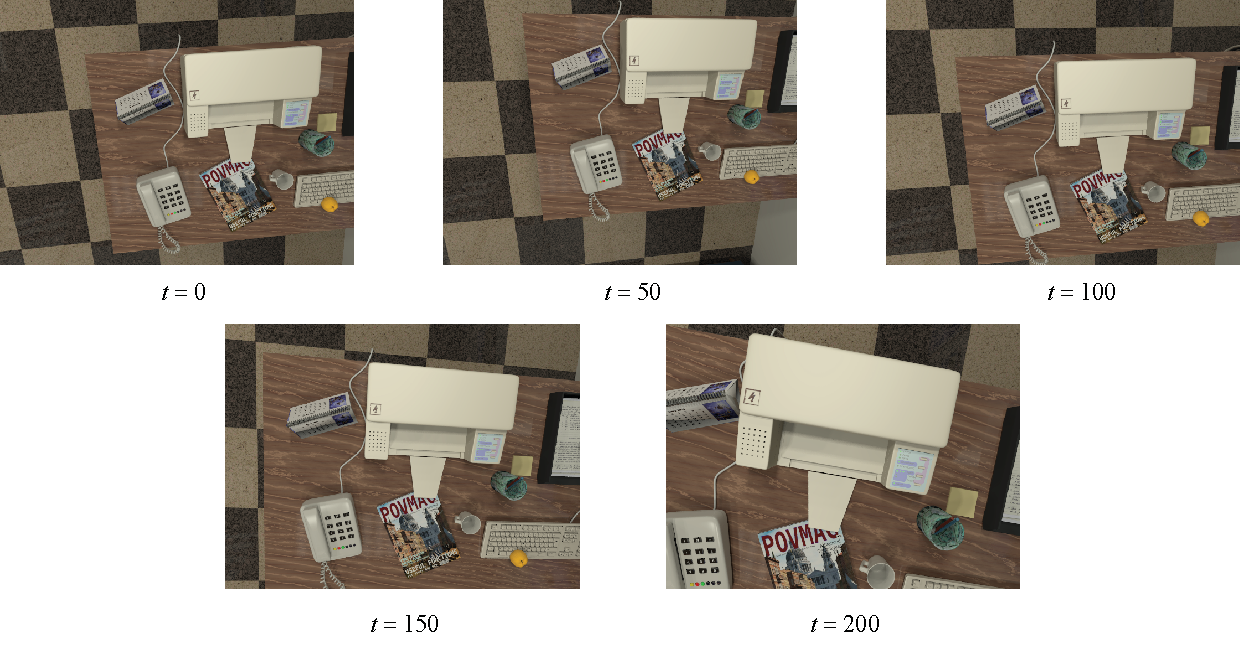
\includegraphics[width=1.0\textwidth]{mapping/remode-dataset.pdf}
	\caption{Sample images from the dataset.}
	\label{fig:remode-dataset}
\end{figure}

\begin{lstlisting}[language=c++,caption=slambook2/ch12/dense\_monocular/dense\_mapping.cpp (part)]
/**********************************************
* This program demonstrates the dense depth estimation of a monocular camera under a known trajectory
* use epipolar search + NCC matching method, which corresponds to section 12.2 of the book
* Please note that this program is not perfect, you can improve it by yourself.
***********************************************/

// ------------------------------------------------------------------
// parameters
const int boarder = 20;         // image boarder
const int width = 640;          // image width
const int height = 480;         // image height
const double fx = 481.2f;       // camera intrinsicss
const double fy = -480.0f;
const double cx = 319.5f;
const double cy = 239.5f;
const int ncc_window_size = 3;    // half window size of NCC 
const int ncc_area = (2 * ncc_window_size + 1) * (2 * ncc_window_size + 1); // area of NCC
const double min_cov = 0.1;     // converge criteria: minimal covariance
const double max_cov = 10;      // disconverge criteria: maximal covariance 

// ------------------------------------------------------------------
// important functions
/**
* update depth using new images
* @param ref           refernce image 
* @param curr          current image 
* @param T_C_R         matrix from ref to cur
* @param depth         depth estimation 
* @param depth_cov     covariance of depth 
* @return              true if success
*/
bool update(
	const Mat &ref, const Mat &curr, const SE3d &T_C_R,
	Mat &depth, Mat &depth_cov2);

/**
* epipolar search
* @param ref           refernce image 
* @param curr          current image 
* @param T_C_R         matrix from ref to cur 
* @param pt_ref        point in ref
* @param depth_mu      mean of depth 
* @param depth_cov     cov of depth 
* @param pt_curr       point in current
* @param epipolar_direction  
* @return              true if success
*/
bool epipolarSearch(
	const Mat &ref, const Mat &curr, const SE3d &T_C_R,
	const Vector2d &pt_ref, const double &depth_mu, const double &depth_cov,
	Vector2d &pt_curr, Vector2d &epipolar_direction);

/**
* update depth filter
* @param pt_ref    point in ref
* @param pt_curr   point in cur 
* @param T_C_R     matrix from ref to cur 
* @param epipolar_direction 
* @param depth     mean of depth 
* @param depth_cov2    cov of depth 
* @return          true if success
*/
bool updateDepthFilter(
	const Vector2d &pt_ref, const Vector2d &pt_curr, const SE3d &T_C_R,
	const Vector2d &epipolar_direction, Mat &depth, Mat &depth_cov2);

/**
* NCC computation
* @param ref       reference image
* @param curr      current image 
* @param pt_ref    reference pixel 
* @param pt_curr   current pixel 
* @return          NCC score
*/
double NCC(const Mat &ref, const Mat &curr, const Vector2d &pt_ref, const Vector2d &pt_curr);

// bilinear interpolation
inline double getBilinearInterpolatedValue(const Mat &img, const Vector2d &pt) {
	uchar *d = &img.data[int(pt(1, 0)) * img.step + int(pt(0, 0))];
	double xx = pt(0, 0) - floor(pt(0, 0));
	double yy = pt(1, 0) - floor(pt(1, 0));
	return ((1 - xx) * (1 - yy) * double(d[0]) +
	xx * (1 - yy) * double(d[1]) +
	(1 - xx) * yy * double(d[img.step]) +
	xx * yy * double(d[img.step + 1])) / 255.0;
}

int main(int argc, char **argv) {
	if (argc != 2) {
		cout << "Usage: dense_mapping path_to_test_dataset" << endl;
		return -1;
	}
	
	// read data
	vector<string> color_image_files;
	vector<SE3d> poses_TWC;
	Mat ref_depth;
	bool ret = readDatasetFiles(argv[1], color_image_files, poses_TWC, ref_depth);
	if (ret == false) {
		cout << "Reading image files failed!" << endl;
		return -1;
	}
	cout << "read total " << color_image_files.size() << " files." << endl;
	
	// first image
	Mat ref = imread(color_image_files[0], 0);                // gray-scale image
	SE3d pose_ref_TWC = poses_TWC[0];
	double init_depth = 3.0;    // initial depth 
	double init_cov2 = 3.0;     // initial covariance 
	Mat depth(height, width, CV_64F, init_depth);             // depth image
	Mat depth_cov2(height, width, CV_64F, init_cov2);         // depth cov image
	
	for (int index = 1; index < color_image_files.size(); index++) {
		cout << "*** loop " << index << " ***" << endl;
		Mat curr = imread(color_image_files[index], 0);
		if (curr.data == nullptr) continue;
		SE3d pose_curr_TWC = poses_TWC[index];
		SE3d pose_T_C_R = pose_curr_TWC.inverse() * pose_ref_TWC;   // T_C_W * T_W_R = T_C_R
		update(ref, curr, pose_T_C_R, depth, depth_cov2);
		evaludateDepth(ref_depth, depth);
		plotDepth(ref_depth, depth);
		imshow("image", curr);
		waitKey(1);
	}
	
	cout << "estimation returns, saving depth map ..." << endl;
	imwrite("depth.png", depth);
	cout << "done." << endl;
	
	return 0;
}


bool update(const Mat &ref, const Mat &curr, const SE3d &T_C_R, Mat &depth, Mat &depth_cov2) {
	for (int x = boarder; x < width - boarder; x++)
	for (int y = boarder; y < height - boarder; y++) {
		if (depth_cov2.ptr<double>(y)[x] < min_cov || depth_cov2.ptr<double>(y)[x] > max_cov) {
			// converge or abort
			continue;
		}
		// search match of (x,y) along the epipolar line
		Vector2d pt_curr;
		Vector2d epipolar_direction;
		bool ret = epipolarSearch(
		ref, curr, T_C_R, Vector2d(x, y), depth.ptr<double>(y)[x],           sqrt(depth_cov2.ptr<double>(y)[x]), pt_curr, epipolar_direction);
		
		if (ret == false) // failed
			continue;
		
		// un-comment this to display the match result 
		// showEpipolarMatch(ref, curr, Vector2d(x, y), pt_curr);
		
		// update if succeed
		updateDepthFilter(Vector2d(x, y), pt_curr, T_C_R, epipolar_direction, depth, depth_cov2);
	}
}


bool epipolarSearch(
	const Mat &ref, const Mat &curr,
	const SE3d &T_C_R, const Vector2d &pt_ref,
	const double &depth_mu, const double &depth_cov,
	Vector2d &pt_curr, Vector2d &epipolar_direction) {
	Vector3d f_ref = px2cam(pt_ref);
	f_ref.normalize();
	Vector3d P_ref = f_ref * depth_mu;    // reference vector
	
	Vector2d px_mean_curr = cam2px(T_C_R * P_ref); // pixel according to mean depth
	double d_min = depth_mu - 3 * depth_cov, d_max = depth_mu + 3 * depth_cov;
	if (d_min < 0.1) d_min = 0.1;
	Vector2d px_min_curr = cam2px(T_C_R * (f_ref * d_min));    // pixel of minimal depth
	Vector2d px_max_curr = cam2px(T_C_R * (f_ref * d_max));    // pixel of maximal depth
	
	Vector2d epipolar_line = px_max_curr - px_min_curr;    // epipolar line
	epipolar_direction = epipolar_line;        // normalized
	epipolar_direction.normalize();
	double half_length = 0.5 * epipolar_line.norm();    
	if (half_length > 100) half_length = 100;   // we don'e want to search too much
	
	// un-comment this to show the epipolar line
	// showEpipolarLine( ref, curr, pt_ref, px_min_curr, px_max_curr );
	
	// epipolar search
	double best_ncc = -1.0;
	Vector2d best_px_curr;
	for (double l = -half_length; l <= half_length; l += 0.7) { // l+=sqrt(2)
		Vector2d px_curr = px_mean_curr + l * epipolar_direction;  
		if (!inside(px_curr))
			continue;
		// compute NCC score
		double ncc = NCC(ref, curr, pt_ref, px_curr);
		if (ncc > best_ncc) {
			best_ncc = ncc;
			best_px_curr = px_curr;
		}
	}
	if (best_ncc < 0.85f)      // only trust NCC with high scores
		return false;
	pt_curr = best_px_curr;
	return true;
}

double NCC(
	const Mat &ref, const Mat &curr,
	const Vector2d &pt_ref, const Vector2d &pt_curr) {
	// zero-mean NCC
	// compute the mean
	double mean_ref = 0, mean_curr = 0;
	vector<double> values_ref, values_curr;
	for (int x = -ncc_window_size; x <= ncc_window_size; x++)
	for (int y = -ncc_window_size; y <= ncc_window_size; y++) {
		double value_ref = double(ref.ptr<uchar>(int(y + pt_ref(1, 0)))[int(x + pt_ref(0, 0))]) / 255.0;
		mean_ref += value_ref;
		
		double value_curr = getBilinearInterpolatedValue(curr, pt_curr + Vector2d(x, y));
		mean_curr += value_curr;
		
		values_ref.push_back(value_ref);
		values_curr.push_back(value_curr);
	}
	
	mean_ref /= ncc_area;
	mean_curr /= ncc_area;
	
	// compute Zero mean NCC
	double numerator = 0, demoniator1 = 0, demoniator2 = 0;
	for (int i = 0; i < values_ref.size(); i++) {
		double n = (values_ref[i] - mean_ref) * (values_curr[i] - mean_curr);
		numerator += n;
		demoniator1 += (values_ref[i] - mean_ref) * (values_ref[i] - mean_ref);
		demoniator2 += (values_curr[i] - mean_curr) * (values_curr[i] - mean_curr);
	}
	return numerator / sqrt(demoniator1 * demoniator2 + 1e-10);  
}

bool updateDepthFilter(
	const Vector2d &pt_ref, const Vector2d &pt_curr, const SE3d &T_C_R,
	const Vector2d &epipolar_direction, Mat &depth, Mat &depth_cov2) {
	// anybody still reading?
	// tri-angulation
	SE3d T_R_C = T_C_R.inverse();
	Vector3d f_ref = px2cam(pt_ref);
	f_ref.normalize();
	Vector3d f_curr = px2cam(pt_curr);
	f_curr.normalize();
	
	// equation:
	// d_ref * f_ref = d_cur * ( R_RC * f_cur ) + t_RC
	// f2 = R_RC * f_cur
	// convert to this:
	// => [ f_ref^T f_ref, -f_ref^T f2 ] [d_ref]   [f_ref^T t]
	//    [ f_cur^T f_ref, -f2^T f2    ] [d_cur] = [f2^T t   ]
	Vector3d t = T_R_C.translation();
	Vector3d f2 = T_R_C.so3() * f_curr;
	Vector2d b = Vector2d(t.dot(f_ref), t.dot(f2));
	Matrix2d A;
	A(0, 0) = f_ref.dot(f_ref);
	A(0, 1) = -f_ref.dot(f2);
	A(1, 0) = -A(0, 1);
	A(1, 1) = -f2.dot(f2);
	Vector2d ans = A.inverse() * b;
	Vector3d xm = ans[0] * f_ref;           // result in ref
	Vector3d xn = t + ans[1] * f2;          // result in cur 
	Vector3d p_esti = (xm + xn) / 2.0;      // take average as p
	double depth_estimation = p_esti.norm();   // depth
	
	// compute the covariance
	Vector3d p = f_ref * depth_estimation;
	Vector3d a = p - t;
	double t_norm = t.norm();
	double a_norm = a.norm();
	double alpha = acos(f_ref.dot(t) / t_norm);
	double beta = acos(-a.dot(t) / (a_norm * t_norm));
	Vector3d f_curr_prime = px2cam(pt_curr + epipolar_direction);
	f_curr_prime.normalize();
	double beta_prime = acos(f_curr_prime.dot(-t) / t_norm);
	double gamma = M_PI - alpha - beta_prime;
	double p_prime = t_norm * sin(beta_prime) / sin(gamma);
	double d_cov = p_prime - depth_estimation;
	double d_cov2 = d_cov * d_cov;
	
	// Gaussian fusion
	double mu = depth.ptr<double>(int(pt_ref(1, 0)))[int(pt_ref(0, 0))];
	double sigma2 = depth_cov2.ptr<double>(int(pt_ref(1, 0)))[int(pt_ref(0, 0))];
	
	double mu_fuse = (d_cov2 * mu + sigma2 * depth_estimation) / (sigma2 + d_cov2);
	double sigma_fuse2 = (sigma2 * d_cov2) / (sigma2 + d_cov2);
	
	depth.ptr<double>(int(pt_ref(1, 0)))[int(pt_ref(0, 0))] = mu_fuse;
	depth_cov2.ptr<double>(int(pt_ref(1, 0)))[int(pt_ref(0, 0))] = sigma_fuse2;
	
	return true;
}
\end{lstlisting}

We omit functions such as drawing and reading data, and only show the part related to the calculation depth. If the reader understands the content of the previous section, I believe it is not difficult to understand the source code here. Nevertheless, we will briefly explain several key functions:
\begin{enumerate}
	\item The main function is very simple. It is only responsible for reading the image from the data set, and then handing it over to the update function to update the depth map.
	\item In the update function, we traverse each pixel of the reference frame, first look for an epipolar match in the current frame, and if it can match, use the result of the epipolar match to update the estimation of the depth map.
	\item The principle of  epipolar search is roughly the same as the one introduced in the previous section, but some details have been added to the implementation: because the depth value is assumed to obey the Gaussian distribution, we take the mean value as the center, and take $\pm 3 \sigma$ as the radius, and then look for the projection of the epipolar line in the current frame. Then, traverse the pixels on this epipolar line (the step size is approximately 0.7 of $\sqrt{2}/2$), and find the point with the highest NCC as the matching point. If the highest NCC is also lower than the threshold (here taken as 0.85), the match is considered failed.
	The calculation of \item NCC uses the method of de-averaging, that is, for the image block $\bm{A}, \bm{B}$, take:
	\begin{equation}
		\mathrm{NCC}_{z} (\bm{A}, \bm{B}) = \frac{{\sum\limits_{i,j} {\left( {\bm{A}(i,j )-\bm{\bar{ A}}(i,j)} \right)\left( {\bm{B}(i,j)-\bm{\bar {B}}(i,j)} \right)} }}{{\sqrt {\sum\limits_{i,j} {{{\left( {\bm{A}(i,j)-\bm{\bar {A}}(i, j)} \right)}^2}} \sum\limits_{i,j} {{{\left( {\bm{B}(i,j)-\bm{\bar {B}}(i, j)} \right)}^2}}} }}.
	\end{equation}
	\item The calculation method of  triangulation is consistent with section 7.5, and the calculation of uncertainty is consistent with the Gaussian fusion method and the previous section.
\end{enumerate}

Although the program is a bit long, I believe readers can understand it according to the above tips. Let's take a look at its actual operation effect.

\subsection*{Experimental results}
After compiling this program, run it with the data set directory as the parameter: \footnote{Please note that the dense depth estimation is time-consuming. If your computer is older, please wait patiently for a while. }
\begin{lstlisting}[language=sh,caption=Terminal ouptut:]
$ build/dense_mapping ~/dataset/test_data 
read total 202 files.
*** loop 1 ***
*** loop 2 ***
......
\end{lstlisting}

The information output by the program is relatively concise, only showing the number of iterations, current image and depth map. Regarding the depth map, we show the result of multiplying the depth value by 0.4-that is, the depth of the pure white point (the value is 1.0) is about 2.5 meters. The darker the color, the smaller the depth value, that is, the closer the object is to us. . If you actually run the program, you should find that the depth estimation is a dynamic process-a process of gradually converging from an uncertain initial value to a stable value. Our initial value used a distribution with a mean and variance of 3.0. Of course, you can also modify the initial distribution to see how it affects the results.

From \autoref{fig:snapshot}~ it can be found that when the number of iterations exceeds a certain value, the depth map becomes stable and no more changes are made to the new data. Observing the stabilized depth map, we find that the difference between the floor and the table can be roughly seen, and the depth of the object on the table is close to that of the table. Most of the entire estimate is correct, but there are also a lot of wrong estimates. They appear as inconsistencies between the depth map and the surrounding data, which are too large or too small estimates. In addition, the place located at the edge, because the number of times seen during the movement is less, so it is not correctly estimated. In summary, we believe that most of the depth map is correct, but it did not achieve the desired effect. We will analyze the causes of these situations in the next section and discuss what can be improved.


\begin{figure}[!ht]
	\centering
	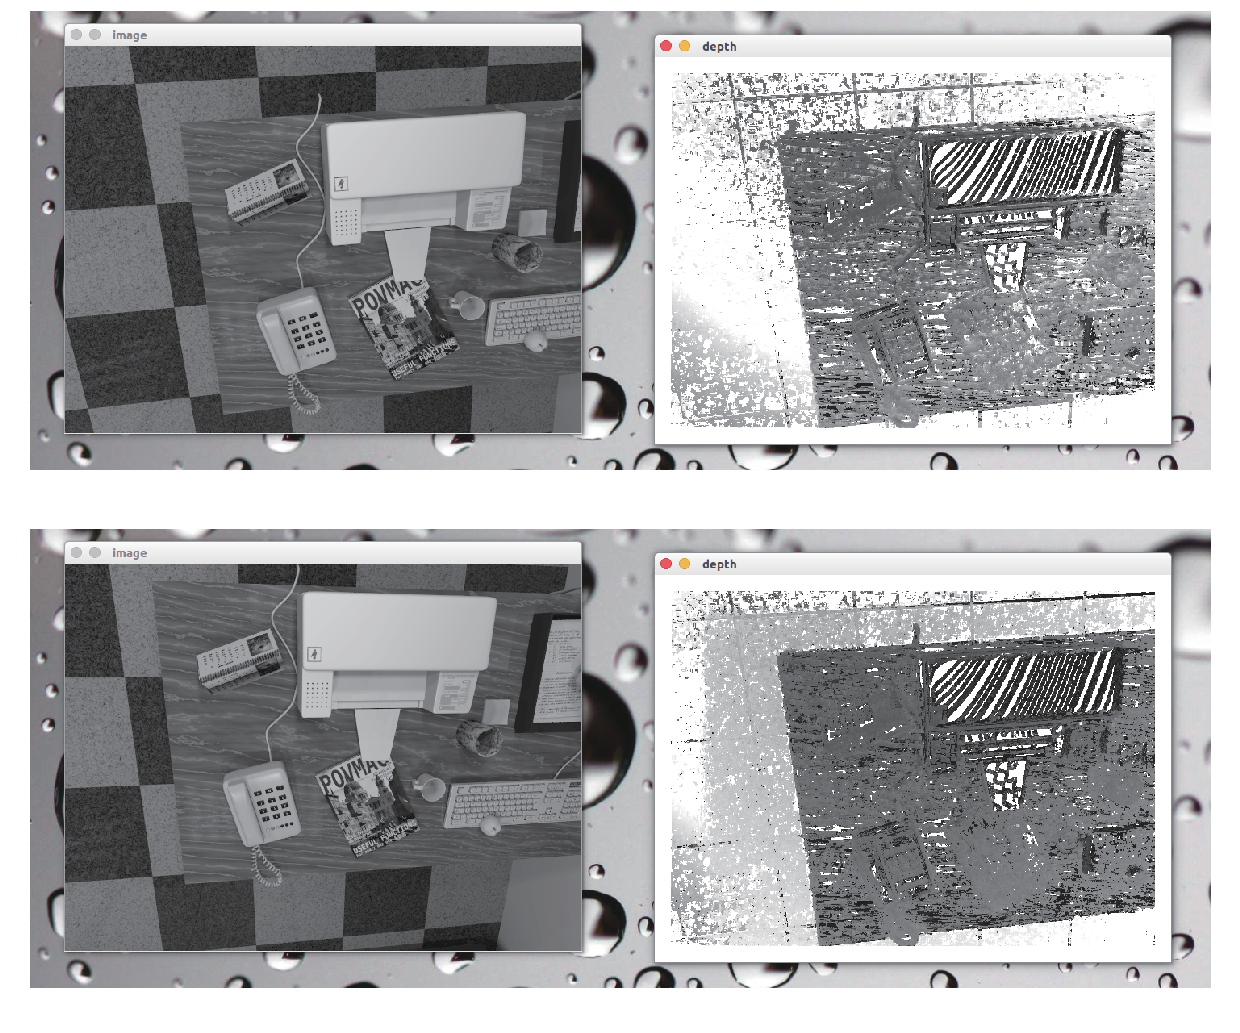
\includegraphics[width=.9\textwidth]{mapping/snapshot.pdf}
	\caption{Snapshots of running the depth filter after 10 and 30 iterations. }
	\label{fig:snapshot}
\end{figure}

\subsection{Discussion}
In the previous section, we demonstrated the dense mapping of a mobile monocular camera and estimated the depth of each pixel of the reference frame. Our code is relatively simple and straightforward, without using many tricks, so there is a common situation in actual engineering-simple is often not the most effective.

Due to the complexity of real data, programs that can work in a real environment often require careful consideration and a lot of engineering skills, which makes every practical code extremely complicated-they are difficult to explain to beginners, so We had to use a less effective, but relatively easy to read and write implementation. Of course, we can put forward several suggestions for improving the demo program, but we do not intend to present the modified (very complicated) program directly to the reader.

Below we conduct a preliminary analysis of the results of the experiment in the previous section. We will analyze the results of the demonstration experiment from the perspective of computer vision and filters.

\subsection{Pixel Gradients}
Observing the depth image, we will find an obvious fact. Whether the block matching is correct or not depends on whether the image block is distinguishable. Obviously, if the image block is only a piece of black or a piece of white, and lacks effective information, then in the NCC calculation, we may erroneously match it with some surrounding pixels. Readers are invited to observe the printer surface in the demo program. Because it is uniform white, it is very easy to cause mismatches, so the depth information on the surface of the printer is mostly incorrect-the spatial surface of the sample program has obviously undesirable striped depth estimates, and according to our intuitive imagination, The surface of the printer must be smooth.

This involves a problem, which we have seen once in the direct method. When performing block matching (and calculation of NCC), we must assume that the small block is unchanged, and then compare the small block with other small blocks. At this time, the small blocks with \textbf{obvious gradient} will have good discrimination and will not easily cause mismatches. For \textbf{pixels with inconspicuous gradients}, since there is no discrimination in block matching, it is difficult for us to effectively estimate its depth. Conversely, where the pixel gradient is more obvious, the depth information we get is relatively accurate, such as magazines, phones and other objects with obvious \textbf{texture} on the desktop. Therefore, the demo program reflects a very common problem in stereo vision: \textbf{dependence on object texture}. This problem is also extremely common in binocular vision, which shows that the reconstruction quality of stereo vision is very dependent on the environment texture.

Our demo program deliberately uses a better-textured environment, such as a checkerboard-like floor, a wood-grained desktop, etc., so we can get a seemingly good result. However, in practice, places with uniform brightness such as walls and smooth surfaces will often appear, affecting our depth estimation. From a certain perspective, the problem is \textbf{cannot be improved and solved on the existing algorithm flow}-if we still only care about the neighborhood (small block) around a certain pixel.

Further discussing the pixel gradient problem, we will also find the connection between the pixel gradient and the epipolar line. The literature \cite{Engel2013} has discussed their relationship in detail, but it is also intuitively reflected in our demo program.

Taking \autoref{fig:epipolar-gradient}~ as an example, we will cite two more extreme cases: the pixel gradient is parallel to the epipolar direction and perpendicular to the epipolar direction. Let's look at the vertical situation first. In the vertical example, even if the small blocks have obvious gradients, when we do block matching along the epipolar line, we will find that the matching degree is the same, so no effective matching can be obtained. Conversely, in the parallel example, we can accurately determine where the highest matching point appears. In reality, the gradient and the epipolar line are probably somewhere in between: they are neither completely vertical nor completely parallel. At this time, we say that when the angle between the pixel gradient and the epipolar line is large, the uncertainty of the epipolar line matching is large; and when the angle is small, the uncertainty of the matching becomes smaller. In the demo program, we uniformly treat these conditions as a pixel error, which is actually not fine enough. After considering the relationship between the epipolar line and the pixel gradient, a more accurate uncertainty model should be used. Specific adjustments and improvements are left as exercises.

\begin{figure}[!htp]
	\centering
	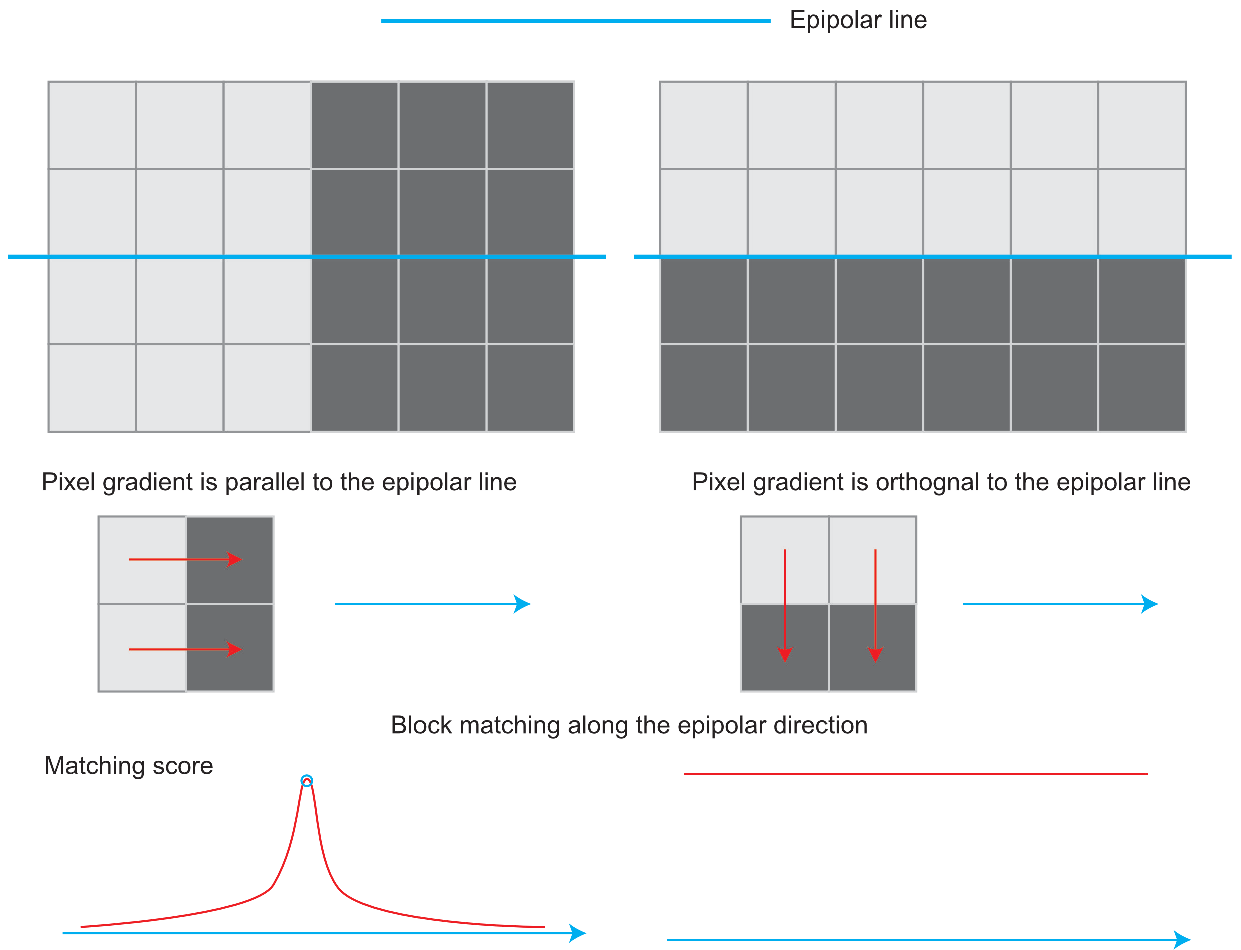
\includegraphics[width=1.0\textwidth]{mapping/epipolar-gradient.pdf}
	\caption{Relationship of pixel gradients and the epipolar direction.}
	\label{fig:epipolar-gradient}
\end{figure}

\subsection{Inverse Depth Filter}
From another perspective, we might as well ask: Is it appropriate to assume that the pixel depth is a Gaussian distribution? This is related to a \textit{parameterization} problem.

In the previous content, we often use the world coordinates $x, y, z$ of a point to describe it, which is a form of parameterization. We think that the three quantities $x, y, z$ are random, and they obey the (three-dimensional) Gaussian distribution. However, this lecture uses the image coordinates $u,v$ and the depth value $d$ to describe a certain spatial point (that is, dense mapping). We think that $u,v$ do not move, and $d$ obeys (one-dimensional) Gaussian distribution, which is another form of parameterization. Then we have to ask: Is there any difference between these two parameterized forms? Can we also assume that $u,v$ obey Gaussian distribution, thus forming another parameterized form?

Different parameterized forms actually describe the same quantity, that is, a certain three-dimensional space point. Considering that when we see a certain point on the camera, its image coordinates $u,v$ are relatively certain. The uncertainty of \footnote{$u,v$ depends on the resolution of the image. }, and the depth value $d$ is very uncertain. At this time, if the world coordinates $x,y,z$ are used to describe this point, then according to the current pose of the camera, there may be an obvious correlation between the three quantities $x,y,z$. Reflected in the covariance matrix, the non-diagonal elements are not zero. And if a point is parameterized with $u, v, d$, then its $u, v$ and $d$ are at least approximately independent, and we can even think that $u, v$ are also independent—thus it The covariance matrix of is approximately diagonal, which is more concise.

Inverse depth is a widely used parameterization technique {\cite{Montiel2006, Civera2008}} that has appeared in SLAM research in recent years. In the demo program, we assume that the depth value satisfies the Gaussian distribution: $d \sim N(\mu, \sigma^2)$. But is it reasonable to do so? Does the depth really approximate a Gaussian distribution? Thinking about it carefully, there are indeed some problems with the normal distribution of depth:

\begin{enumerate}
	\item What we actually want to express is: the depth of this scene is about 5\textasciitilde10 meters, there may be some further points, but the close distance will definitely not be less than the camera focal length (or think that the depth will not be less than 0). This distribution does not form a symmetrical shape like the Gaussian distribution. Its tail may be slightly longer, and the negative area is zero.
	\item In some outdoor applications, there may be points that are very far away, or even at infinity. It is difficult to cover these points in our initial value, and there will be some numerical difficulties in describing them with Gaussian distribution.
\end{enumerate}

Thus, the inverse depth came into being. People found in the simulation that the hypothesis that the reciprocal of the depth, which is \textbf{inverse depth}, is a Gaussian distribution, which is more effective {\cite{Civera2008}}. Later, in practical applications, the inverse depth also has better numerical stability, which gradually becomes a general technique, which exists in the standard practice in the existing SLAM scheme {\cite{Forster2014, Engel2014, Mur- Artal2015}}.

It is not complicated to change the demonstration program from positive depth to inverse depth. Just change $d$ to the inverse depth $d^{-1}$ in the derivation of the previous depth. We also leave this change as an exercise for readers to complete.

\subsection{Image Pre-transform}
Before block matching, it is also a common preprocessing method to do a transformation from image to image. This is because we assume that image patches remain unchanged when the camera is moving, and this assumption can be maintained when the camera is shifted (the example data set is basically such an example), but when the camera rotates significantly, It is difficult to continue. In particular, when the camera rotates around the optical center, an image that is black and white on the bottom may become a black and white image block on top, causing the correlation to directly become a negative number (although it is still the same block).

In order to prevent this situation, we usually need to compare the reference frame with the current frame before block matching.
\begin{equation}
	d_R {\bm{P}_R} = \bm{K} \left( {{\bm{R}_{\mathrm{RW}}}{\bm{P}_W} + {\bm{t}_{\mathrm{RW}}}} \right).
\end{equation}

Similarly, for the current frame, there is a projection of $\bm{P}_W$ on it, denoted as $\bm{P}_C$:
\begin{equation}
	d_C {\bm{P}_C} = \bm{K} \left( {{\bm{R}_{\mathrm{CW}}}{\bm{P}_W} + {\bm{t}_{\mathrm{CW}}}} \right).
\end{equation}

Substituting and eliminating $\bm{P}_W$, the pixel relationship between the two images is obtained:
\begin{equation}
	d_C {\bm{P}_C} = d_R \bm{K} \bm{R}_{\mathrm{CW}} \bm{R}_{\mathrm{RW}}^\mathrm{T} \bm{K}^{-1} \bm{P}_R + \bm{K} \bm{t}_{\mathrm{CW}} - \bm{K} \bm{R}_{\mathrm{CW}} \bm{R}_{\mathrm{RW}}^\mathrm{T} \bm{K} \bm{t}_{\mathrm{RW}}.
\end{equation}

When we know $d_R, \bm{P}_R$, we can calculate the projection position of $\bm{P}_C$. At this time, give the two components of $\bm{P}_R$ an increment $\mathrm{d}u, \mathrm{d}v$, then the increment of $\bm{P}_C$ can be obtained. Quantity $\mathrm{d}u_c, \mathrm{d}v_c$. In this way, a linear relationship between the coordinate transformation of the reference frame and the current frame image in a local range is calculated to form an affine transformation:
\begin{equation}
	\left[ \begin{array}{l}
		\mathrm{d}u_c\\
		\mathrm{d}v_c
	\end{array} \right] = \left[ {\begin{array}{*{20}{c}}
			{\frac{{\mathrm{d}u_c}}{{\mathrm{d}u}}}&{\frac{{\mathrm{d}u_c}}{{\mathrm{d}v}}}\\
			{\frac{{\mathrm{d}v_c}}{{\mathrm{d}u}}}&{\frac{{\mathrm{d}v_c}}{{\mathrm{d}v}}}
	\end{array}} \right]\left[ \begin{array}{l}
		\mathrm{d}u\\
		\mathrm{d}v
	\end{array} \right]
\end{equation}

According to the affine transformation matrix, we can transform the pixels of the current frame (or reference frame) and then perform block matching, in order to obtain a better effect on rotation.

\subsection{Parallel Computing}
In the experiment, we have also seen that the estimation of the dense depth map is very time-consuming. This is because the points we want to estimate have changed from the original hundreds of feature points to hundreds of thousands of pixels. Even now mainstream CPUs It is impossible to calculate such a huge amount in real time. However, the problem also has another nature: the depth estimates of these hundreds of thousands of pixels are independent of each other! This makes parallelization useful.

In the sample program, we traverse all the pixels in a double loop, and perform epipolar search on them one by one. When we use the CPU, this process is carried out serially: the calculation of the next pixel must be completed after the previous pixel is calculated. However, in fact, there is no need for the next pixel to wait for the calculation of the previous pixel to end, because there is no obvious connection between them, so we can use multiple threads to calculate each pixel separately, and then unify the results. Theoretically, if we have 300,000 threads, the calculation time for this problem is the same as calculating one pixel.

The parallel computing architecture of GPU is very suitable for such problems. Therefore, in the dense reconstruction of single, double and binocular, it is often seen that the GPU is used for parallel acceleration. Of course, this book is not going to involve GPU programming, so we only point out the possibility of using GPU acceleration here, and the specific practice is left to the reader as a verification. According to some similar work, the dense depth estimation using GPU can be real-time on mainstream GPU.

\subsection{Other Improvements}
In fact, we can also propose many improvements to this example, such as:

\begin{enumerate}
	\item Now each pixel is completely calculated independently. There may be cases where the depth of this pixel is small and the next one is large. We can assume that the adjacent depth changes in the depth map will not change too much, thus adding a spatial regularization term to the depth estimation. This approach will make the resulting depth map smoother.
	\item We did not explicitly deal with the case of Outlier. In fact, due to various factors such as occlusion, lighting, motion blur, etc., it is impossible to maintain a successful match for every pixel. In the practice of the demonstration program, as long as the NCC is greater than a certain value, it is considered that a successful match has occurred, and the mismatch is not considered.
	To
	There are also several ways to handle mismatches. For example, the depth filter under the uniform-Gaussian mixture distribution proposed in the document \cite{Vogiatzis2011} explicitly distinguishes the interior points from the exterior points and performs probabilistic modeling, which can better process the exterior point data. However, this type of filter theory is more complicated, and this book does not want to involve too much, readers can read the original paper.
\end{enumerate}

As can be seen from the above discussion, there are many possible improvements. If we carefully improve every step of the way, we can hope to get a good dense mapping plan in the end. However, as we discussed, there are some problems \textbf{with theoretical difficulties}, such as the dependence on the environment texture, and the correlation between the pixel gradient and the epipolar direction (and the parallel case). These problems are \textbf{difficult to solve by adjusting the code}. So, until now, although binoculars and mobile monoculars can build dense maps, we usually think that they rely too much on environmental textures and lighting and are not reliable enough.

\section{Dense RGB-D Mapping}
In addition to using monocular and binocular for dense reconstruction, RGB-D cameras are a better choice within the scope of application. The depth estimation problem discussed in detail in the last lecture can be obtained by hardware measurement in the sensor in an RGB-D camera, without consuming a lot of computing resources to estimate. In addition, the structured light or time-of-flight principle of RGB-D ensures that the depth data is independent of texture. Even when facing a solid-colored object, as long as it can reflect light, we can measure its depth. This is also a major advantage of RGB-D sensors.

It is relatively easy to use RGB-D for dense mapping. However, depending on the map format, there are also several different mainstream mapping methods. The most intuitive and easiest method is to convert the RGB-D data into a point cloud (Point Cloud) based on the estimated camera pose, and then stitch, and finally get a Point Cloud Map composed of discrete points. ). On this basis, if we have further requirements for the appearance and want to estimate the surface of the object, we can use the triangular mesh (Mesh) and the surface (Surfel) to build the map. On the other hand, if you want to know the obstacle information of the map and navigate on the map, you can also create an Occupancy Map through voxel.

We seem to have introduced many new concepts. Please don't worry, readers, we will introduce them one by one slowly. For some suitable experiments, we will also provide several demonstration programs as usual. Since there is not much theoretical knowledge involved in RGB-D mapping, the following sections will directly introduce the practical part. GPU mapping is beyond the scope of this book, so we will briefly explain its principles and will not demonstrate.

\subsection{Practice: RGB-D Point Cloud Mapping}
First, let's explain the simplest point cloud map. The so-called point cloud is a map represented by a set of discrete points. The most basic point contains three-dimensional coordinates of $x, y, z$, and can also contain color information of $r, g, b$. Since the RGB-D camera provides a color map and a depth map, it is easy to calculate the RGB-D point cloud based on the camera's internal parameters. If the pose of the camera is obtained by some means, then as long as the point clouds are directly added, the global point cloud can be obtained. In the ~\ref{sec:join-point-cloud}~ section of this book, an example of splicing point clouds through camera internal and external parameters was given. However, that example is mainly for the reader to understand the internal and external parameters of the camera, and in the actual mapping, we will also add some filtering processing to the point cloud to obtain a better visual effect. In this program, we mainly use two kinds of filters: the outer point removal filter, and the voxel grid filter (Voxel grid filter). The code of the sample program is as follows (because part of the code is the same as before, we mainly look at the changed part):

\begin{lstlisting}[language=c++,caption=slambook/ch12/dense\_RGBD/pointcloud\_mapping.cpp (part)]
int main(int argc, char **argv) {
	vector<cv::Mat> colorImgs, depthImgs;   
	vector<Eigen::Isometry3d> poses;       
	
	ifstream fin("./data/pose.txt");
	if (!fin) {
		cerr << "cannot find pose file" << endl;
		return 1;
	}
	
	for (int i = 0; i < 5; i++) {
		boost::format fmt("./data/%s/%d.%s"); // we use boost::format to read image files
		colorImgs.push_back(cv::imread((fmt % "color" % (i + 1) % "png").str()));
		depthImgs.push_back(cv::imread((fmt % "depth" % (i + 1) % "png").str(), -1)); // use -1 to read the unchanged data
		
		double data[7] = {0};
		for (int i = 0; i < 7; i++) {
			fin >> data[i];
		}
		Eigen::Quaterniond q(data[6], data[3], data[4], data[5]);
		Eigen::Isometry3d T(q);
		T.pretranslate(Eigen::Vector3d(data[0], data[1], data[2]));
		poses.push_back(T);
	}
	
	// merge the point clouds
	// intrinsics
	double cx = 319.5;
	double cy = 239.5;
	double fx = 481.2;
	double fy = -480.0;
	double depthScale = 5000.0;
	
	cout << "convering image to point cloud ..." << endl;
	
	// use XYZRGB as our format
	typedef pcl::PointXYZRGB PointT;
	typedef pcl::PointCloud<PointT> PointCloud;
	
	PointCloud::Ptr pointCloud(new PointCloud);
	for (int i = 0; i < 5; i++) {
		PointCloud::Ptr current(new PointCloud);
		cout << "converting " << i + 1 << endl;
		cv::Mat color = colorImgs[i];
		cv::Mat depth = depthImgs[i];
		Eigen::Isometry3d T = poses[i];
		for (int v = 0; v < color.rows; v++)
		for (int u = 0; u < color.cols; u++) {
			unsigned int d = depth.ptr<unsigned short>(v)[u]; // depth data
			if (d == 0) continue; // 0 means invalid reading 
			Eigen::Vector3d point;
			point[2] = double(d) / depthScale;
			point[0] = (u - cx) * point[2] / fx;
			point[1] = (v - cy) * point[2] / fy;
			Eigen::Vector3d pointWorld = T * point;
			
			PointT p;
			p.x = pointWorld[0];
			p.y = pointWorld[1];
			p.z = pointWorld[2];
			p.b = color.data[v * color.step + u * color.channels()];
			p.g = color.data[v * color.step + u * color.channels() + 1];
			p.r = color.data[v * color.step + u * color.channels() + 2];
			current->points.push_back(p);
		}
		// depth filter and statistical removal 
		PointCloud::Ptr tmp(new PointCloud);
		pcl::StatisticalOutlierRemoval<PointT> statistical_filter;
		statistical_filter.setMeanK(50);
		statistical_filter.setStddevMulThresh(1.0);
		statistical_filter.setInputCloud(current);
		statistical_filter.filter(*tmp);
		(*pointCloud) += *tmp;
	}
	
	pointCloud->is_dense = false;
	cout << "we have " << pointCloud->size() << " points." << endl;
	
	// voxel filter 
	pcl::VoxelGrid<PointT> voxel_filter;
	double resolution = 0.03;
	voxel_filter.setLeafSize(resolution, resolution, resolution);       // resolution
	PointCloud::Ptr tmp(new PointCloud);
	voxel_filter.setInputCloud(pointCloud);
	voxel_filter.filter(*tmp);
	tmp->swap(*pointCloud);
	
	cout << "Now we have " << pointCloud->size() << " points after voxel filtering." << endl;
	
	pcl::io::savePCDFileBinary("map.pcd", *pointCloud);
	return 0;
}
\end{lstlisting}

This code needs to install the point cloud library. In Ubuntu 18.04, just one command is enough:
\begin{lstlisting}[language=sh, caption=Terminal input:]
	sudo apt-get install libpcl-dev pcl-tools
\end{lstlisting}

The code does not change much comparing with that in the fifth lecture。 The main differences are:
\begin{enumerate}
	\item When generating the point cloud of each frame, remove the points with invalid depth values. This is mainly because of the effective range of Kinect, the depth value after exceeding the range will have a large error or return a zero.
	\item Use statistical filter method to remove outliers. This filter counts the distribution of the distance value between each point and the nearest $N$ point, and removes the points whose distance is too large. In this way, we keep those "sticky" points and remove isolated noise points.
	\item Finally, the voxel network filter is used for downsampling. Due to the overlapping of multiple viewing angles, there will be a large number of points that are very similar in the overlapping area. This will take up a lot of memory space in vain. Voxel filtering ensures that there is only one point in a certain size cube (or voxel), which is equivalent to downsampling the three-dimensional space, which can save a lot of storage space.
\end{enumerate}

In the second edition of the book, we use the ICL-NUIM dataset as an example. This data set is a simulated RGB-D data set, which allows us to get noise-free depth data to facilitate experiments. We store five images and depth maps, and the corresponding camera poses in the data/ directory. In the voxel filter, we set the resolution to 0.03, which means that there is only one point in each grid of 0.03$\times$0.03$\times$0.03. This is a relatively high resolution, so we can't feel the difference in the map in practice, but we can see from the program output that the number of points has been significantly reduced (from 1.3 million points to 30,000 points, only 2$ \%$ storage space).

Execute in the dense\_RGBD directory:
\begin{lstlisting}[language=sh, caption=Terminal input:]
	./build/pointcloud_mapping
\end{lstlisting}
The point cloud file map.pcd can be obtained in the same directory. Then, open the pcd with the pcl\_viewer tool, you can see the content, as shown in \autoref{fig:pcd-filter}.

\begin{figure}[!ht]
	\centering
	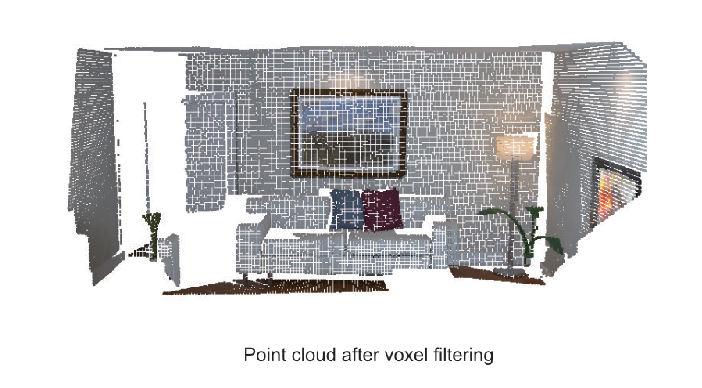
\includegraphics[width=1.0\textwidth]{mapping/pcd-filter.pdf}
	\caption{Point cloud mapping using five image paris in ICL-NUIM.}
	\label{fig:pcd-filter}
\end{figure}

The point cloud map provides us with a relatively basic visual map, allowing us to roughly understand what the environment looks like. It is stored in three dimensions, allowing us to quickly browse all corners of the scene and even roam in the scene. A big advantage of point clouds is that they can be efficiently generated directly from RGB-D images without additional processing. Its filtering operation is also very intuitive, and the processing efficiency is acceptable. However, the use of point clouds to express maps is still very elementary. We might as well follow the requirements for maps mentioned earlier to see if point cloud maps can meet.

\begin{enumerate}
	\item Localization requirements: depends on the processing method of the front-end visual odometer. If it is a visual odometer based on feature points, because there is no feature point information stored in the point cloud, it cannot be used in a feature point-based positioning method. If the front end is the ICP of the point cloud, then you can consider ICP for the local point cloud to the global point cloud to estimate the pose. However, this requires the global point cloud to have better accuracy. In our way of processing point clouds, the point cloud itself is not optimized, so it is not enough.
	\item Requirements for navigation and obstacle avoidance: Cannot be used directly for navigation and obstacle avoidance. A pure point cloud cannot express the information of "whether there is an obstacle", nor can we make queries such as "whether any spatial point is occupied" in the point cloud, which is the basic need for navigation and obstacle avoidance. However, it can be processed on the basis of point clouds to obtain a map format that is more suitable for navigation and obstacle avoidance.
	\item Visualization and interaction: Basic visualization and interaction capabilities. We can see the appearance of the scene, and we can also walk through the scene. From the perspective of visualization, since the point cloud only contains discrete points and no surface information (such as normals), it does not conform to people's visualization habits. For example, the object of a point cloud map is the same from the front and the back, and you can see what is behind it through the object: these are not in line with our daily experience.
\end{enumerate}

In summary, we say that the point cloud map is "basic" or "primary", which means that it is closer to the raw data read by the sensor. It has some basic functions, but it is usually used for debugging and basic display, which is inconvenient to use directly in applications. If we want the map to have more advanced functions, the point cloud map is a good starting point. For example, for the navigation function, we can start from the point cloud to construct an Occupancy Grid for the navigation algorithm to query whether a point can pass. Another example is the Poisson reconstruction {\cite{Kazhdan2006}} method commonly used in SfM, which can reconstruct the object mesh map from the basic point cloud to obtain the surface information of the object. In addition to Poisson reconstruction, Surfel is also a way to express the surface of an object. Using facets as the basic unit of the map, it can build a beautiful visual map {\cite{Stuckler2014}}.

\autoref{fig:poisson-surfel}~ shows an example of Poisson reconstruction and Surfel. It can be seen that their visual effects are significantly better than pure point cloud mapping, and they can all be constructed through point clouds. Most of the map formats obtained from point cloud conversion are provided in the PCL library, and interested readers can further explore the contents of the PCL library. As this book serves as an introductory material, it does not introduce every map form in detail.

\begin{figure}[!htp]
	\centering
	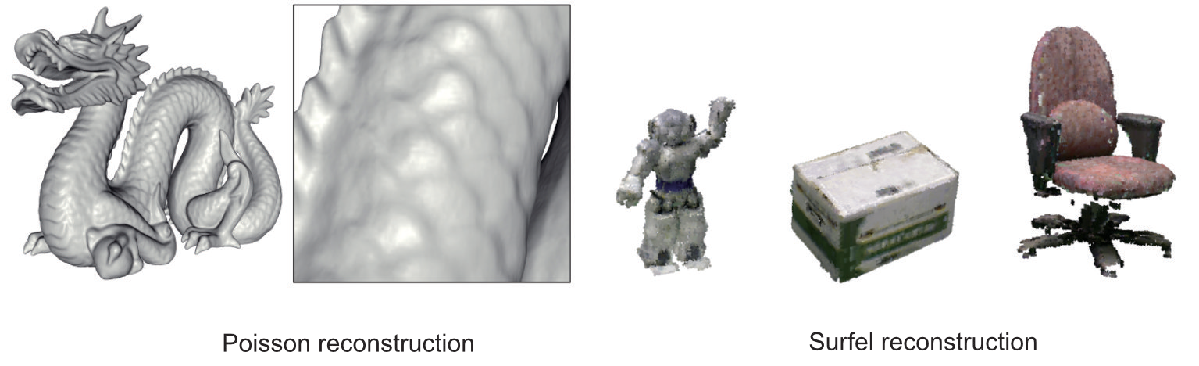
\includegraphics[width=1.0\textwidth]{mapping/poisson-surfel.pdf}
	\caption{Reconstruction results of Poisson and surfel model. }
	\label{fig:poisson-surfel}
\end{figure}

\subsection{Building Meshes from Point Cloud}
Reconstructing the mesh from the point cloud is also relatively easy. Let's demonstrate how to build the mesh based on the point cloud file just now. The general idea is: first calculate the normal of the point cloud, and then calculate the grid from the normal.

\begin{lstlisting}[language=c++,caption=slambook2/ch12/dense_RGBD/surfel_mapping.cpp]
#include <pcl/point_cloud.h>
#include <pcl/point_types.h>
#include <pcl/io/pcd_io.h>
#include <pcl/visualization/pcl_visualizer.h>
#include <pcl/kdtree/kdtree_flann.h>
#include <pcl/surface/surfel_smoothing.h>
#include <pcl/surface/mls.h>
#include <pcl/surface/gp3.h>
#include <pcl/surface/impl/mls.hpp>

// typedefs
typedef pcl::PointXYZRGB PointT;
typedef pcl::PointCloud<PointT> PointCloud;
typedef pcl::PointCloud<PointT>::Ptr PointCloudPtr;
typedef pcl::PointXYZRGBNormal SurfelT;
typedef pcl::PointCloud<SurfelT> SurfelCloud;
typedef pcl::PointCloud<SurfelT>::Ptr SurfelCloudPtr;

SurfelCloudPtr reconstructSurface(
const PointCloudPtr &input, float radius, int polynomial_order) {
	pcl::MovingLeastSquares<PointT, SurfelT> mls;
	pcl::search::KdTree<PointT>::Ptr tree(new pcl::search::KdTree<PointT>);
	mls.setSearchMethod(tree);
	mls.setSearchRadius(radius);
	mls.setComputeNormals(true);
	mls.setSqrGaussParam(radius * radius);
	mls.setPolynomialFit(polynomial_order > 1);
	mls.setPolynomialOrder(polynomial_order);
	mls.setInputCloud(input);
	SurfelCloudPtr output(new SurfelCloud);
	mls.process(*output);
	return (output);
}

pcl::PolygonMeshPtr triangulateMesh(const SurfelCloudPtr &surfels) {
	// Create search tree*
	pcl::search::KdTree<SurfelT>::Ptr tree(new pcl::search::KdTree<SurfelT>);
	tree->setInputCloud(surfels);
	
	// Initialize objects
	pcl::GreedyProjectionTriangulation<SurfelT> gp3;
	pcl::PolygonMeshPtr triangles(new pcl::PolygonMesh);
	
	// Set the maximum distance between connected points (maximum edge length)
	gp3.setSearchRadius(0.05);
	
	// Set typical values for the parameters
	gp3.setMu(2.5);
	gp3.setMaximumNearestNeighbors(100);
	gp3.setMaximumSurfaceAngle(M_PI / 4); // 45 degrees
	gp3.setMinimumAngle(M_PI / 18); // 10 degrees
	gp3.setMaximumAngle(2 * M_PI / 3); // 120 degrees
	gp3.setNormalConsistency(true);
	
	// Get result
	gp3.setInputCloud(surfels);
	gp3.setSearchMethod(tree);
	gp3.reconstruct(*triangles);
	
	return triangles;
}

int main(int argc, char **argv) {
	// Load the points
	PointCloudPtr cloud(new PointCloud);
	if (argc == 0 || pcl::io::loadPCDFile(argv[1], *cloud)) {
		cout << "failed to load point cloud!";
		return 1;
	}
	cout << "point cloud loaded, points: " << cloud->points.size() << endl;
	
	// Compute surface elements
	cout << "computing normals ... " << endl;
	double mls_radius = 0.05, polynomial_order = 2;
	auto surfels = reconstructSurface(cloud, mls_radius, polynomial_order);
	
	// Compute a greedy surface triangulation
	cout << "computing mesh ... " << endl;
	pcl::PolygonMeshPtr mesh = triangulateMesh(surfels);
	
	cout << "display mesh ... " << endl;
	pcl::visualization::PCLVisualizer vis;
	vis.addPolylineFromPolygonMesh(*mesh, "mesh frame");
	vis.addPolygonMesh(*mesh, "mesh");
	vis.resetCamera();
	vis.spin();
}
\end{lstlisting}

This program demonstrates the process of calculating normals and meshes. Use:
\begin{lstlisting}[language=sh,caption=Terminal input:]
	./build/surfel_mapping map.pcd
\end{lstlisting}
to convert the point cloud into a grid map, as shown in \autoref{fig:mesh}. It can be seen that after the mesh is reconstructed, the normal, texture and other information can be constructed from the point cloud without surface information. For the point cloud reconstruction algorithms (Moving Least Square and Greedy Projection) demonstrated in this section, readers can find them in the literature \cite{Alexa2003} and \cite{Marton2009}, which are relatively classic reconstruction algorithms.

\begin{figure}[!htp]
	\centering
	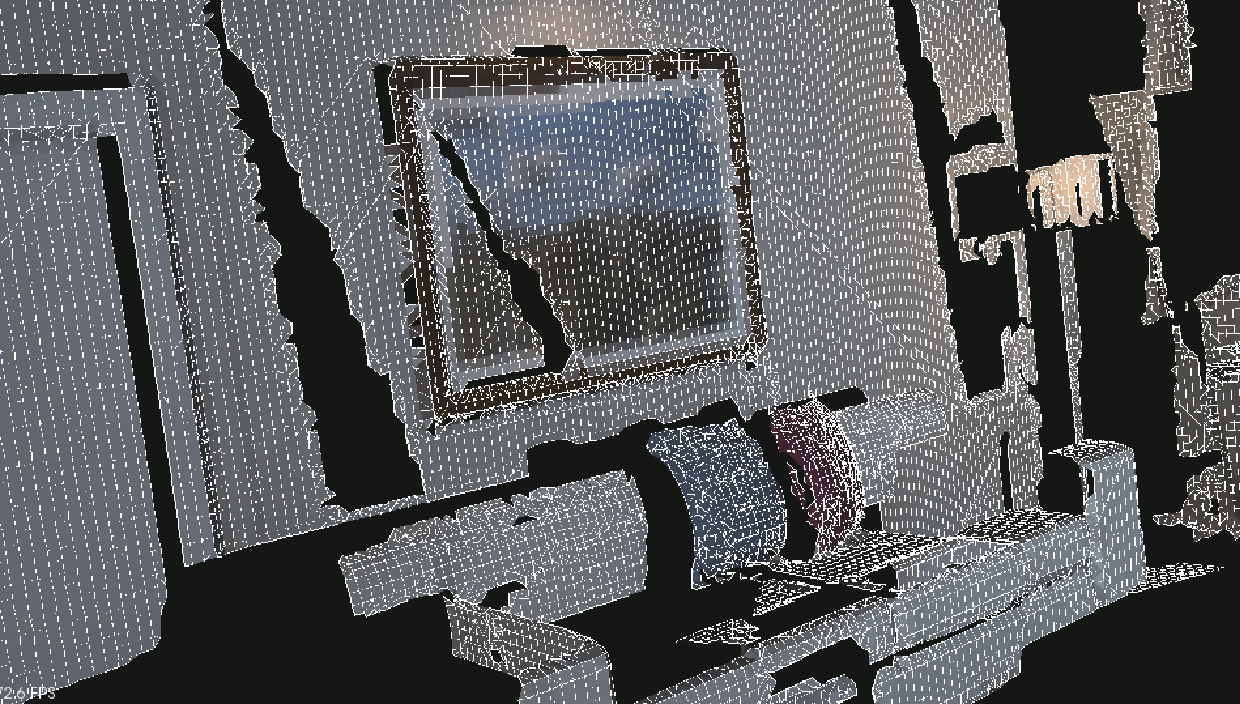
\includegraphics[width=1.0\textwidth]{mapping/mesh.pdf}
	\caption{Building meshes from point clouds.}
	\label{fig:mesh}
\end{figure}

\subsection{Octo-Mapping}
The following introduces a map format that is commonly used in navigation and has better compression performance: \textbf{octree map}. In the point cloud map, although we have a three-dimensional structure and voxel filtering to adjust the resolution, the point cloud has several obvious defects:
\begin{itemize}
	\item The point cloud map is usually very large, so the pcd file will be very large. An image of $640$pixel$\times480$pixel will generate 300,000 spatial points and require a lot of storage space. Even after some filtering, the pcd file is very large. And the annoying thing is that its "big" is not necessary. Point cloud maps provide a lot of unnecessary details. Regarding the folds on the carpet and the shadows in the shadows, we do not particularly care about these things. Putting them on the map is a waste of space. Due to the occupation of these spaces, unless we reduce the resolution, it is impossible to model a larger environment with limited memory. However, reducing the resolution will cause the quality of the map to decrease. Is there any way to compress and store the map and discard some duplicate information?
	\item The point cloud map cannot handle moving objects. Because our approach is only "add points", and there is no "remove points when they disappear" approach. In the actual environment, the ubiquity of moving objects makes point cloud maps not practical enough.
\end{itemize}

And what we are going to introduce next is a flexible, compressed, and updateable map format: octo-map {\cite{Hornung2013}}.

We know that it is a common practice to model three-dimensional space as many small squares (or voxels). If we cut each face of a small square into two pieces on average, then this small square will become eight small squares of the same size. This step can be repeated continuously until the final square size reaches the highest accuracy of modeling. In this process, the matter of "dividing a small square into eight of the same size" is regarded as "expanding from one node into eight child nodes", then the whole process of subdividing from the largest space to the smallest space is an octo-tree.

As shown in \autoref{fig:octomap}~, the left side shows a large cube continuously divided into eight pieces evenly until it becomes the smallest square. Therefore, the entire large square can be regarded as the root node, and the smallest block can be regarded as the "leaf node". Therefore, in the octree, when we move up one level from the next level of nodes, the volume of the map can be expanded to eight times the original. We might as well do a simple calculation: if the square size of the leaf node is 1 cm$^3$, then when we limit the octree to 10 levels, the total volume that can be modeled is about $8^{10}\text{ cm}^3 = 1,073\text{m}^3$, which is enough to model a room. Since volume and depth have an exponential relationship, when we use greater depth, the modeled volume will grow very fast.

\begin{figure}[!ht]
	\centering
	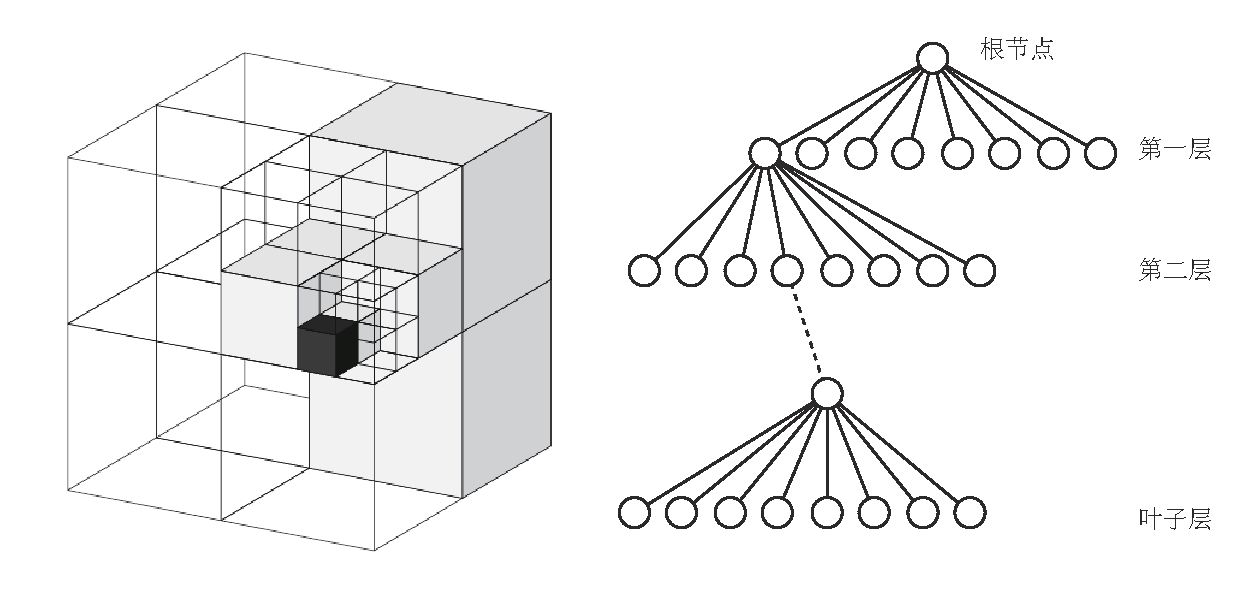
\includegraphics[width=1.0\textwidth]{mapping/octomap.pdf}
	\caption{The structure of an octo-tree.}
	\label{fig:octomap}
\end{figure}

Readers may be wondering, in the voxel filter of the point cloud, don't we also limit a voxel to only one point? Why do we say that the point cloud takes up space, while the octree saves space? This is because, in the octree, we store information about whether it is occupied or not in the node. However, the difference is that when all child nodes of a block are occupied or not occupied, then there is \textbf{no need to expand this node}. For example, when the map is blank at the beginning, we only need a root node instead of a complete tree. When adding information to the map, since actual objects are often connected together, and blank places are often connected together, most octree nodes do not need to be expanded to the leaf level. So, octree saves a lot of storage space than point cloud.

As mentioned earlier, the nodes of the octree store information about whether it is occupied. From the point cloud level, we can naturally use 0 for blank and 1 for occupied. This 0−1 representation can be stored in one bit, saving space, but it seems a bit too simple. Due to the influence of noise, we may see a certain point as 0 for a while and 1 for a while; or 0 for most of the time and 1 for a small amount of time; or in addition to the two cases of "yes" and "no", there are An "unknown" state. Can you describe this in more detail? We will choose to use the form of \textbf{probability} to express whether a node is occupied. For example, use a floating point number $x \in [0,1]$ to express. This $x$ takes 0.5 at the beginning. If you keep observing that it is occupied, let this value keep increasing; on the contrary, if you keep observing that it is blank, let it keep decreasing.

In this way, we dynamically model the obstacle information in the map. However, the current method has a small problem: if $x$ is kept increasing or decreasing, it may go outside the range of $[0,1]$, causing inconvenience in processing. So we do not directly use probability to describe a certain node being occupied, but use log-odds to describe it. Let $y \in \mathbb{R}$ be the logarithmic value of the probability and $x$ be the probability of 0\textasciitilde1, then the transformation between them is described by the logit transformation:
\begin{equation}
	y = \mathrm{logit}(x) = \log \left( \frac{x}{1-x} \right).
\end{equation}

The inverse transform is:
\begin{equation}
	x = \mathrm{logit}^{-1}(y) = \frac{\exp(y)}{\exp(y)+1}.
\end{equation}

It can be seen that when $y$ changes from $-\infty$ to $+\infty$, $x$ changes from 0 to 1 accordingly. When $y$ takes 0, $x$ takes 0.5. Therefore, we might as well store $y$ to express whether the node is occupied. When "occupation" is continuously observed, let $y$ increase by one value; otherwise, let $y$ decrease by one value. When querying the probability, use the inverse logit transformation to convert $y$ to probability. In mathematical terms, suppose a certain node is $n$, and the observed data is $z$. Then the logarithm value of the probability of a node from the beginning to the moment $t$ is $L(n|z_{1:t})$, and the time $t+1$ is:
\begin{equation}
	L(n|z_{1:t+1}) = L(n|z_{1:t-1}) + L(n|z_{t}).
\end{equation}

If written in probabilistic form instead of logarithmic form of probability, it would be a bit more complicated:
\begin{equation}
	P(n|z_{1:T}) =  \left[ 1+ \frac{1-P(n|z_T)}{P(n|z_T)} \frac{1-P(n|z_{1:T-1})}{P(n|z_{1:T-1})} \frac{P(n)}{1-P(n)} \right]^{-1}.
\end{equation}

With logarithmic probability, we can update the entire octree map based on RGB-D data. Suppose we observe a certain pixel with depth $d$ in the RGB-D image, which shows one thing: we \textbf{ observe an occupancy data at the spatial point corresponding to the depth value, and from the camera light The line segment from which the mind starts to this point should be without objects} (otherwise it will be blocked). With this information, the octree map can be updated well and the structure of the movement can be processed.

\subsection{Practice: Octo-mapping}
Let's demonstrate the process of octo-mapping through the program. Please install the octomap library first. After 18.04, octomap and the corresponding visualization tool octovis have been integrated in apt and can be installed by the following command:
\begin{lstlisting}[language=sh,caption=Terminal input:]
	sudo apt-get install liboctomap-dev octovis
\end{lstlisting}
We will directly demonstrate how to generate an octree map from the previous 5 images, and then draw it with octovis.
\begin{lstlisting}[language=c++,caption=slambook/ch13/dense\_RGBD/octomap\_mapping.cpp (part)]
// octomap tree 
octomap::OcTree tree(0.01); // resolution=0.01

for (int i = 0; i < 5; i++) {
	cout << "Converting " << i + 1 << endl;
	cv::Mat color = colorImgs[i];
	cv::Mat depth = depthImgs[i];
	Eigen::Isometry3d T = poses[i];
	
	octomap::Pointcloud cloud;  // the point cloud in octomap 
	
	for (int v = 0; v < color.rows; v++)
	for (int u = 0; u < color.cols; u++) {
		unsigned int d = depth.ptr<unsigned short>(v)[u]; 
		if (d == 0) continue; 
		Eigen::Vector3d point;
		point[2] = double(d) / depthScale;
		point[0] = (u - cx) * point[2] / fx;
		point[1] = (v - cy) * point[2] / fy;
		Eigen::Vector3d pointWorld = T * point;
		cloud.push_back(pointWorld[0], pointWorld[1], pointWorld[2]);
	}
	
	// save into octo tree
	tree.insertPointCloud(cloud, octomap::point3d(T(0, 3), T(1, 3), T(2, 3)));
}

// update and save into a bt file
tree.updateInnerOccupancy();
cout << "saving octomap ... " << endl;
tree.writeBinary("octomap.bt");
\end{lstlisting}

We used octomap::OcTree to build the entire map. In fact, octomap provides many kinds of octrees: some with maps and some with occupancy information. You can also define which variables each node needs to carry. For simplicity, we used the most basic octree map without color information.

A point cloud structure is provided inside Ocotmap. It is slightly simpler than the point cloud of PCL, and only carries the spatial position information of the point. According to the RGB-D image and camera pose information, we first transfer the coordinates of the point to the world coordinates, then put it into the point cloud of octomap, and finally give it to the octree map. After that, octomap will update the internal occupation probability according to the projection information introduced before, and finally save it as a compressed octree map. We save the generated map as octomap.bt file. When octovis was compiled before, we actually installed a visualization program, namely octovis. Now, call it to open the map file, and you can see the actual map.

\autoref{fig:octomap-result}~ shows the result of the map we built. Since we did not add color information to the map, it will be gray when opening the map at the beginning. Press the "1" key to color it according to the height information. Readers can get familiar with the operation interface of octovis, including map viewing, rotation, zooming, etc.

\begin{figure}[!htp]
	\centering
	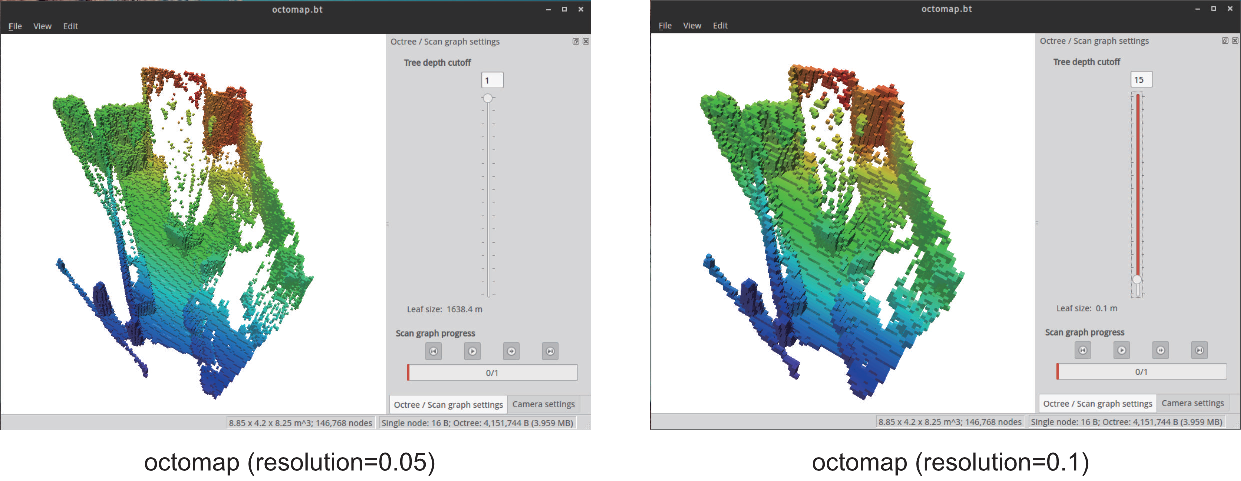
\includegraphics[width=1.0\textwidth]{mapping/octomap-result.pdf}
	\caption{The display results of the octree map at different resolutions.}
	\label{fig:octomap-result}
\end{figure}

There is an octree depth limit bar on the right, where you can adjust the resolution of the map. Since the default depth we used in the construction is 16 layers, the 16 layers are the highest resolution displayed here, that is, the side length of each small block is 0.05 meters. When we reduce the depth by one layer, the leaf nodes of the octree are raised one layer, and the side length of each small block doubles to 0.1 meters. As you can see, we can easily adjust the map resolution to suit different occasions.

Octomap also has some places that can be explored. For example, we can easily query the occupation probability of any point to design a method for navigating in the map {\cite{Burri2015}}. Readers can also compare the file sizes of point cloud maps and octree maps. The disk file of the point cloud map generated in the previous section is about 6.9MB, while the octomap is only 56KB, which is less than one percent of the point cloud map, which can effectively model larger scenes.


\section{\textsuperscript{\ttfamily *} TSDF and RGB-D Fusion Series}
At the end of this lecture, we introduce a research direction that is very similar to SLAM but slightly different: real-time 3D reconstruction. This section involves GPU programming and does not provide reference examples, so it is used as an optional reading material.

In the previous map model, \textbf{with positioning as the main body}. The stitching of the map is placed in the SLAM frame as a subsequent processing step. The reason why this framework has become mainstream is that the positioning algorithm can meet the real-time requirements, and the processing of the map can be processed at the key frame without real-time response. Localization is usually lightweight, especially when using sparse features or sparse direct methods; accordingly, the expression and storage of maps are heavyweight. Their large scale and computational requirements are not conducive to real-time processing. Especially dense maps can only be calculated at the key frame level.

However, in the current practice, we have not optimized the dense map. For example, when the same chair is observed in two images, we only superimpose the point clouds at the two locations based on the poses of the two images to generate a map. Since pose estimation is usually error-prone, this direct stitching is often not accurate enough. For example, the point clouds of the same chair cannot be superimposed together perfectly. At this time, two ghost images of the chair will appear on the map-this phenomenon is sometimes vividly called "ghost shadow".

This phenomenon is obviously not what we want. We hope that the reconstruction result is smooth and complete, in line with our understanding of the map. Under this kind of thinking, there has been a practice of taking "map" as the main body and positioning in a secondary position, which is the real-time 3D reconstruction to be introduced in this section. Since 3D reconstruction takes the reconstruction of an accurate map as the main goal, it basically needs to use GPU for acceleration, and even requires very advanced GPU or multiple GPUs for parallel acceleration, usually requiring heavier computing equipment. In contrast, SLAM is developing towards lightweight and miniaturization. Some solutions even abandon the mapping and loop detection part, and only retain the visual odometer. The real-time reconstruction is developing towards the reconstruction of large-scale and large-scale dynamic scenes.

Since the emergence of RGB-D sensors, real-time reconstruction using RGB-D images has formed an important development direction. Kinect Fusion {\cite{Newcombe2011}} and Dynamic Fusion {\cite{Newcombe2015}} , Elastic Fusion {\cite{Whelan2015}}, Fusion4D {\cite{Dou2016}}, Volumn Deform {\cite{Innmann2016}} and other achievements. Among them, Kinect Fusion has completed the basic model reconstruction, but it is limited to small scenes; the follow-up work is to expand it to large, sports, and even deformed scenes. We regard them as real-time reconstruction of a broad category of work, but due to the large variety, it is impossible to discuss the working principles of each in detail. \autoref{fig:fusions}~ shows part of the reconstruction results. You can see that these modeling results are very fine, much more delicate than simply splicing point clouds.

\begin{figure}[!htp]
	\centering
	\includegraphics[width=0.9\textwidth]{mapping/fusions.pdf}
	\caption{Reconstruction by the fusion series: (a) Kinect Fusion; (b) Dynamic Fusion; (c) Volumn Deform; (d) Fusion4D; (e) Elastic Fusion.}
	\label{fig:fusions}
\end{figure}

We will introduce the classic TSDF map as a representative. TSDF is the abbreviation of Truncated Signed Distance Function, it may be translated as \textbf{Truncation Signed Distance Function}. Although it seems inappropriate to call "function" "map", we will temporarily call it TSDF map, TSDF reconstruction, etc., as long as there is no deviation in understanding until there is a better translation.

Similar to the octree, the TSDF map is also a grid format (or square) map, as shown in \autoref{fig:tsdf}. First select the three-dimensional space to be modeled, such as $3\times3\times3 \text{m}^3$, divide this space into many small blocks according to a certain resolution, and store the information inside each small block. The difference is that the entire TSDF map is stored in video memory instead of memory. Using the parallel feature of GPU, we can compute and update each voxel in parallel, instead of having to serialize as the CPU traverses the memory area.

\begin{figure}[!t]
	\centering
	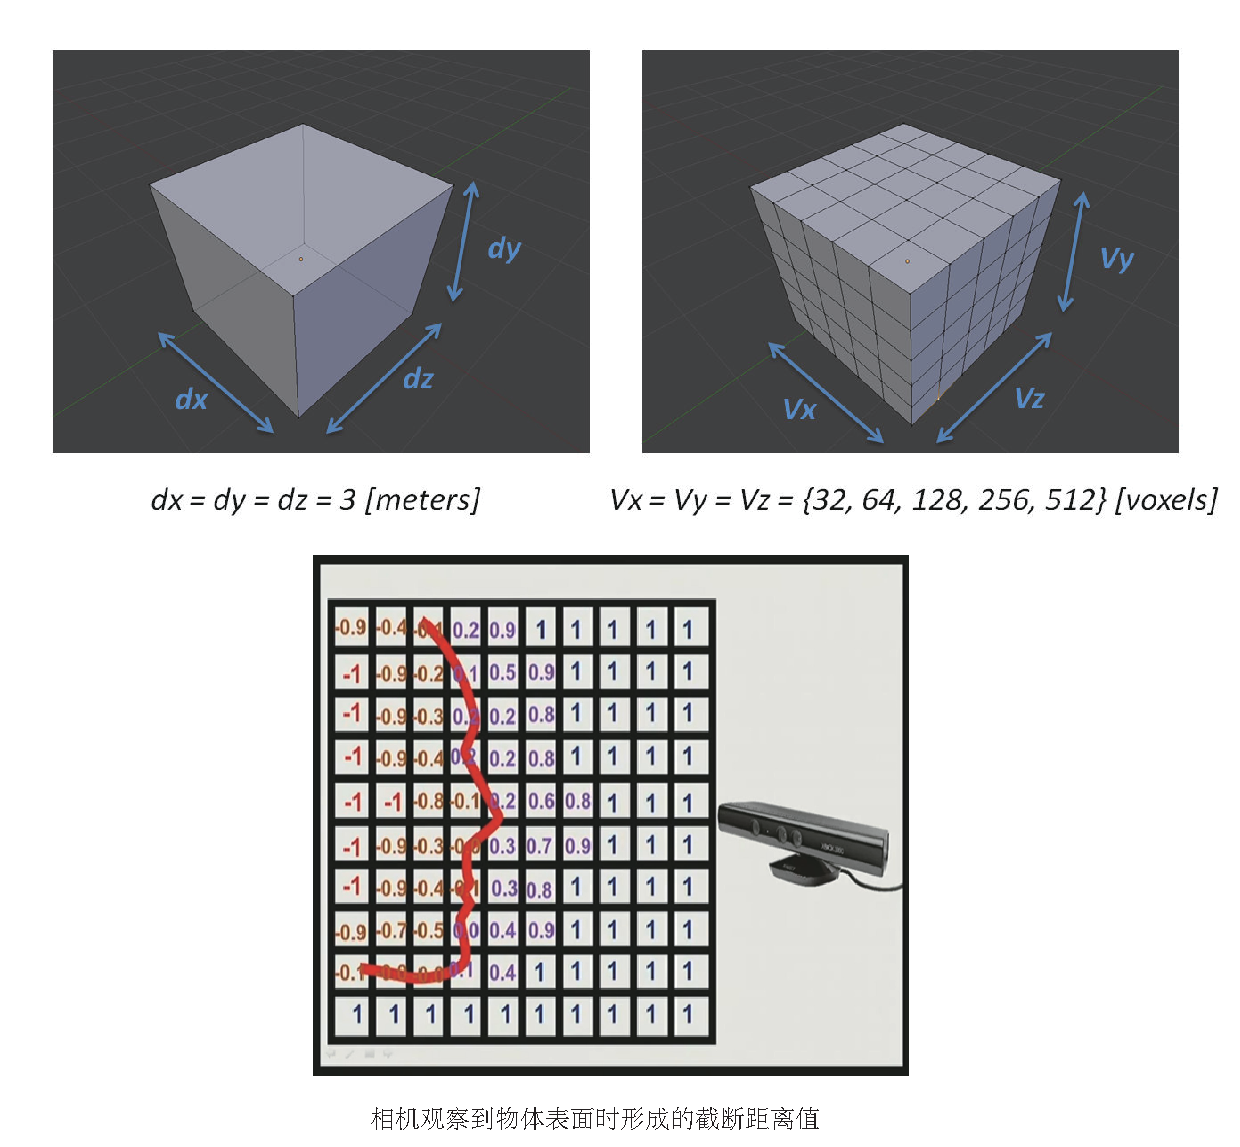
\includegraphics[width=1.0\textwidth]{mapping/tsdf.pdf}
	\caption{Truncation Signed Distance Function.}
	\label{fig:tsdf}
\end{figure}

In each TSDF voxel, the distance between the small block and the surface of the closest object is stored. If the small piece is in front of the surface of the object, it has a positive value; conversely, if the small piece is behind the surface, then it has a negative value. Since the surface of the object is usually a thin layer, the values that are too large and too small are taken as $1$ and $-1$, so that the distance after truncation is obtained, which is the so-called TSDF. So by definition, the place where TSDF is 0 is the surface itself—or, due to the existence of numerical errors, the place where TSDF changes from negative to positive is the surface itself. In the lower part of \autoref{fig:tsdf}~, we see a surface similar to a human face appearing where the TSDF changes sign.

TSDF also has two problems of "localization" and "map building", which are very similar to SLAM, but the specific form is slightly different from the previous lectures in this book. Here, the positioning problem mainly refers to how to compare the current RGB-D image with the TSDF map in the GPU to estimate the camera pose. The problem of mapping is how to update the TSDF map based on the estimated camera pose. In the traditional approach, we also perform a bilateral Bayesian filter on the RGB-D image to remove the noise in the depth map.

The positioning of TSDF is similar to the ICP described earlier, but due to the parallelization of GPU, we can perform ICP calculation on the entire depth map and TSDF map without having to calculate the feature points first like traditional visual odometry. At the same time, because TSDF does not have color information, it means that we can \textbf{only use depth map} and complete pose estimation without using color maps, which to some extent get rid of the dependence of visual mileage calculation method on illumination and texture , Making the RGB-D reconstruction more robust\footnote{But having said that, it is more dependent on the depth map. }. On the other hand, the mapping part is also a process of updating the values ​​in the TSDF in parallel, making the estimated surface smoother and more reliable. Since we do not introduce GPU-related content too much, the specific method will not be elaborated. Please refer to relevant literature for interested readers.

\section{Summary}
This lecture introduces some common map types, especially dense map forms. We see that dense maps can be constructed based on monocular or binocular, while RGB-D maps are often easier and more stable. The map in this lecture focuses on the measurement map, and the topological map form is quite different from the SLAM research, so it is not discussed in detail.

\section*{Exercises}
\begin{enumerate}
	\item Prove (12.6).
	\item Change the dense depth estimation in this lecture to semi-dense, you can first filter out the places with obvious gradients.
	\item[\optional] Change the monocular dense reconstruction code demonstrated in this lecture from positive depth to inverse depth, and add affine transformation. Has the effect of your experiment improved?
	\item Can you demonstrate how to navigate or plan a path in an octree?
	\item Read \cite{Newcombe2011} to discuss how the TSDF map performs pose estimation and update. What are the similarities and differences between it and the positioning mapping algorithm we talked about before?
	\item[\optional] Study the principle and realization of uniform-Gaussian mixture filter.
\end{enumerate}
